\documentclass[spanish,a4paper,12pt,oneside]{extreport}

\usepackage[dvips]{graphicx}
\usepackage[dvips]{epsfig}
\usepackage[utf8]{inputenc}
\usepackage[spanish]{babel}
\usepackage{alltt}

\usepackage[ruled,vlined,commentsnumbered,linesnumbered,inoutnumbered,titlenotnumbered,noend]{algorithm2e}
\SetKwRepeat{Do}{do}{while}

\usepackage{multirow}
\usepackage{array} 
\usepackage{amsfonts}
\usepackage{amsmath}
\usepackage{bigstrut}
\usepackage{booktabs}
\usepackage{caption}
\usepackage{chngpage}
\usepackage{float}
\usepackage{comment}
%\usepackage{enumitem,lipsum}
\usepackage{graphicx}
\usepackage{lscape}
\usepackage{microtype}
\usepackage{natbib}
\usepackage{pdflscape}
\usepackage{rotating}
\usepackage{subcaption}
\usepackage{ctable}
\usepackage{hyperref}
\usepackage{enumerate}
\usepackage{gensymb}
\usepackage{eurosym}
\usepackage{xcolor}
\usepackage{tabu}
\usepackage[export]{adjustbox}[2011/08/13]
\usepackage{lineno}
\usepackage{epigraph}
%\usepackage[sanitize=none]{glossaries}
\usepackage[toc]{glossaries}

%\\linenumbers
%\setlength\linenumbersep{5pt}
%\renewcommand\linenumberfont{\normalfont\tiny\sffamily\color{gray}}

%\makenoidxglossaries
\makeglossaries

\newglossaryentry{DSL}{
    name={DSL},
    description={
        Un lenguaje específico de dominio (DSL) es un lenguaje que está dirigido a resolver un tipo particular de problema. El uso de DSL es muy común en informática: CSS, expresiones regulares, make, ant, SQL, muchos bits de Rails, expectativas en JMock, el lenguaje graphviz, los archivo de configuración de strut, etc.
    }
}

%\newglossaryentry{GitHub Action}{
%    name={GitHub Action},
%    description={
%        GitHub Actions es una plataforma de integración continua y entrega continua (CI/CD) que permite automatizar la %canalización de tareas como la compilación, pruebas y despliegue, permitiendo crear flujos de trabajo que construyan %nuevos artefactos como publicaciones, releases, imágenes, pdfs, etc.
%    }
%}

\newglossaryentry{JIT}
{
    name=JIT,
    description={just-in-time compiler. También conocido en español como \textbf{compilación en tiempo de ejecución}. Es una forma de ejecutar el código informático que implica la compilación durante la ejecución de un programa (en tiempo de ejecución) en lugar de antes de la ejecución}
}

\newglossaryentry{AOT}
{
    name=AOT,
    description={En informática, la \textbf{compilación anticipada} es el acto de compilar un lenguaje de programación (a menudo) de alto nivel en un lenguaje (a menudo) de bajo nivel antes de la ejecución de un programa, normalmente en tiempo de compilación, para reducir la cantidad de trabajo necesario en tiempo de ejecución.
    De hecho, dado que todas las compilaciones estáticas se realizan técnicamente con antelación, esta expresión en particular se utiliza a menudo para destacar algún tipo de ventajas de rendimiento del acto de dicha precompilación. El acto de compilar Java a bytecode Java es por tanto raramente referido como AOT ya que es normalmente un requisito, no una optimización}
}

\newglossaryentry{API}
{
    name=API,
    description={Una \textbf{interfaz de programación de aplicaciones} es una manera de que dos o más programas informáticos se comuniquen entre sí. Es un tipo de interfaz de software que ofrece un servicio a otras piezas de software}
}

\newglossaryentry{power users}
{
    name=power users,
    description={Un \textbf{usuario avanzado} es un usuario de ordenadores, software y otros dispositivos electrónicos, que utiliza características avanzadas del hardware informático, sistemas operativos, programas o sitios web que no son utilizados por el usuario medio. Un usuario avanzado puede no tener amplios conocimientos técnicos de los sistemas que utiliza, pero se caracteriza más bien por la competencia o el deseo de hacer el uso más intensivo de los programas o sistemas informáticos}
}

\newglossaryentry{cache}
{
    name=caché,
    description={Una \textbf{cache} es un componente de hardware o software que almacena datos para que las futuras solicitudes de esos datos puedan ser atendidas más rápidamente; los datos almacenados en una caché pueden ser el resultado de un cálculo anterior o una copia de datos almacenados en otro lugar}
}

\newglossaryentry{CLI}
{
    name=CLI,
    description={Es un tipo de interfaz de usuario de computadora que permite a los usuarios dar instrucciones a algún programa informático o al sistema operativo por medio de una línea de texto simple}
}

\newglossaryentry{strategy pattern}
{
    name=patrón estrategia,
    description={En programación informática, el patrón de estrategia (también conocido como patrón de política) es un patrón de diseño de software de comportamiento que permite seleccionar un algoritmo en tiempo de ejecución. En lugar de implementar un único algoritmo directamente, el código recibe instrucciones en tiempo de ejecución sobre cuál de una familia de algoritmos utilizar}
}

\newglossaryentry{graceful degradation}{
    name={degradación gradual},
    description={La \textbf{tolerancia a los fallos} es la propiedad que permite a un sistema seguir funcionando correctamente en caso de fallo de uno o varios de sus componentes. A diferencia de un sistema diseñado ingenuamente, en el que incluso un pequeño fallo puede provocar una avería total}
}

\newglossaryentry{namespace}{
    name={espacio de nombre},
    description={En informática, un \textbf{espacio de nombres} es un conjunto de signos (nombres) que se utilizan para identificar y referirse a objetos de diversos tipos. Un espacio de nombres garantiza que todos los objetos de un conjunto determinado tengan nombres únicos para que puedan ser fácilmente identificados}
}

\newglossaryentry{corrutine}{
    name={corrutina},
    description={Las \textbf{corrutinas} son componentes de programas informáticos que generalizan las subrutinas para la multitarea no preferente, permitiendo suspender y reanudar la ejecución}
}

\newglossaryentry{hash}{
    name={hash},
    description={Un \textbf{hash} (que también puede llamarse un condensado o una firma) es un valor calculado a partir de un valor diferente. En la gran mayoría de los casos, este valor está representado en forma de una cadena de caracteres hexadecimales. Los hashs suelen utilizarse para verificar que un archivo no se ha visto corrompido o bien para autentificar a un usuario sin tener que almacenar su contraseña en claro}
}

\newglossaryentry{regex}{
    name={expresión regular},
    plural={expresiones regulares},
    description={Una \textbf{expresión regular} (abreviada como regex o regexp) es una secuencia de caracteres que especifica un patrón de búsqueda en un texto. Los algoritmos de búsqueda de cadenas suelen utilizar estos patrones para las operaciones de "búsqueda" o "búsqueda y sustitución" de cadenas, o para la validación de entradas}
}

\newglossaryentry{deserialization}{
    name={deserializar},
    plural={deserializa},
    description={Extraer una estructura de datos de una serie de bytes}
}

\newglossaryentry{serialization}{
    name={serializar},
    plural={serializa},
    description={Es el proceso de traducir una estructura de datos o el estado de un objeto a un formato que pueda ser almacenado (por ejemplo, en un archivo o en un búfer de datos de la memoria) o transmitido (por ejemplo, a través de una red informática)}
}

\usepackage[top=2cm, bottom=2cm, left=2cm, right=2cm]{geometry}

\newenvironment{sourcecode}
{\begin{list}{}{\setlength{\leftmargin}{1em}}\item\scriptsize\bfseries}
{\end{list}}

\newenvironment{littlesourcecode}
{\begin{list}{}{\setlength{\leftmargin}{1em}}\item\tiny\bfseries}
{\end{list}}

\newenvironment{summary}
{\par\noindent\begin{center}\textbf{Abstract}\end{center}\begin{itshape}\par\noindent}
{\end{itshape}}

\newenvironment{keywords}
{\begin{list}{}{\setlength{\leftmargin}{1em}}\item[\hskip\labelsep \bfseries Keywords:]}
{\end{list}}

\newenvironment{palabrasClave}
{\begin{list}{}{\setlength{\leftmargin}{1em}}\item[\hskip\labelsep \bfseries Palabras clave:]}
{\end{list}}

\usepackage{bera}% optional: just to have a nice mono-spaced font
\usepackage{listings}
\usepackage{xcolor}

\colorlet{punct}{red!60!black}
\definecolor{background}{HTML}{EEEEEE}
\definecolor{delim}{RGB}{20,105,176}
\colorlet{numb}{magenta!60!black}

\lstdefinelanguage{json}{
    basicstyle=\normalfont\ttfamily,
    numbers=left,
    numberstyle=\scriptsize,
    stepnumber=1,
    numbersep=8pt,
    showstringspaces=false,
    breaklines=true,
    frame=lines,
    backgroundcolor=\color{background},
    literate=
     *{0}{{{\color{numb}0}}}{1}
      {1}{{{\color{numb}1}}}{1}
      {2}{{{\color{numb}2}}}{1}
      {3}{{{\color{numb}3}}}{1}
      {4}{{{\color{numb}4}}}{1}
      {5}{{{\color{numb}5}}}{1}
      {6}{{{\color{numb}6}}}{1}
      {7}{{{\color{numb}7}}}{1}
      {8}{{{\color{numb}8}}}{1}
      {9}{{{\color{numb}9}}}{1}
      {:}{{{\color{punct}{:}}}}{1}
      {,}{{{\color{punct}{,}}}}{1}
      {\{}{{{\color{delim}{\{}}}}{1}
      {\}}{{{\color{delim}{\}}}}}{1}
      {[}{{{\color{delim}{[}}}}{1}
      {]}{{{\color{delim}{]}}}}{1},
}

% Configuración de los colores de los enlaces
\hypersetup{
    colorlinks = true,
    linkcolor = blue,
    filecolor = magenta,      
    urlcolor = cyan,
}

\begin{document}

\renewcommand\listtablename{Índice de Tablas}    
\renewcommand\listfigurename{Índice de Figuras}    

%%%%%%%%%%%%%%%%%%%%%%%%%%%%%%%%%%%%%%%%%%%%%%%%%%%%%%%%%%%%%%%%%%%%%%%%%%%%%%%
% First Page
%%%%%%%%%%%%%%%%%%%%%%%%%%%%%%%%%%%%%%%%%%%%%%%%%%%%%%%%%%%%%%%%%%%%%%%%%%%%%%%
\pagestyle{empty}
\thispagestyle{empty}


\newcommand{\HRule}{\rule{\linewidth}{1mm}}
\setlength{\parindent}{0mm}
\setlength{\parskip}{0mm}

\vspace*{\stretch{0.5}}

\begin{center}

\includegraphics[scale=0.8]{images/escuela-ingenieria-tecnologia-original}\\[10mm]
{\Huge Trabajo de Fin de Grado}
\end{center}

\HRule
\begin{flushright}
    {\Huge Extending GitHub CLI with Default Owners} \\[2.5mm]
    {\Large \textit Extendiendo GitHub CLI con Propietarios por Defecto} \\[5mm]
    {\Large Diego Pérez García} \\[5mm]
\end{flushright}
\HRule

\vspace*{\stretch{2}}
\begin{center}
  \Large La Laguna, \today
\end{center}

\setlength{\parindent}{5mm}

%%%%%%%%%%%%%%%%%%%%%%%%%%%%%%%%%%%%%%%%%%%%%%%%%%%%%%%%%%
% Signature page (add the official stamp)
%%%%%%%%%%%%%%%%%%%%%%%%%%%%%%%%%%%%%%%%%%%%%%%%%%%%%%%%%%
\newpage
\thispagestyle{empty}

D. {\bf Casiano Rodríguez León}, con N.I.F. 42.020.072-S  profesor Catedrático de Universidad adscrito al Departamento de Nombre del Departamento de la Universidad de La Laguna, como tutor


\bigskip
\bigskip
{\bf C E R T I F I C A N}

\bigskip
\bigskip
Que la presente memoria titulada:

\bigskip
''{\it Extending GitHub CLI with Default Owners}''

\bigskip
\bigskip
\bigskip

\noindent ha sido realizada bajo su dirección por D. {\bf Diego Pérez García},
con N.I.F. 79081733M.

\bigskip
\bigskip

Y para que así conste, en cumplimiento de la legislación vigente y a los efectos
oportunos firman la presente en La Laguna a \today

%%%%%%%%%%%%%%%%%%%%%%%%%%%%%%%%%%%%%%%%%%%%%%%%%%%%%%%%%%
\newpage
\thispagestyle{empty}

%{ \flushright

\begin{LARGE}
Agradecimientos
\end{LARGE}

\hspace{3mm}

\begin{large}
A mis amigos ya graduados que me han brindado apoyo, consejo y ánimos a pesar de haberme tardado un año más que ellos. \\
A mi mejor amiga por brindarme el mayor de los apoyos cuando tuve que repetir asignaturas. \\
A su vez a mis compañeros por esta gran experiencia y esos recuerdos que me llevo de mi vida universitaria. \\
A los profesores Francisco de Sande González, Marcos Colebrook-Santamaria, Iván Castilla Rodríguez y Albano José González Fernández por su gran labor como profesores demostrando cada año que tratan de llegar a los alumnos para transmitir sus conocimientos de la mejor manera. \\
A mi familia que me ha permitido centrarme en los estudios que me han llevado a ser el programador que soy hoy. \\
Y por último a mi tutor Casiano Rodríguez León por ofrecer esta oportunidad de proyecto y aprendizaje, a la vez de ser un profesor con paciencia y que me ha permitido sacar el mejor resultado. \\
\end{large}

%}
%%%%%%%%%%%%%%%%%%%%%%%%%%%%%%%%%%%%%%%%%%%%%%%%%%%%%%%%
\newpage
\thispagestyle{empty}

\bigskip
\begin{LARGE}
Licencia
\end{LARGE}

\begin{center}

\includegraphics[scale=1.8]{images/by_88x31}\\[5mm]
\end{center}

\begin{large}
© Esta obra está bajo una licencia de Creative Commons Reconocimiento 4.0 Internacional.
\end{large}

%%%%%%%%%%%%%%%%%%%%%%%%%%%%%%%%%%%%%%%%%%%%%%%%%%%%%%%%
\newpage 
\thispagestyle{empty}

\begin{abstract} % TODO: Revisar ortografía
Está muy arraigado en la informática el uso de GitHub como plataforma de enseñanza.
Es así que esta promuebe las iniciativas de educación con GitHub Education. Dando paso a herramientas claves como GitHub Classroom con soporte para asignar tareas de manera fácil y sencilla. Por otra parte la plataforma ofrece una herramienta llamada GitHub CLI que permite interactuar con esta atraves de la línea de comandos.

Este trabajo presenta un comando nuevo para la GitHub CLI denominado \verb|gh owner| que tiene como objetivo romper con un problema de experiencia de usuario que es tener que recordar los largos y varios OWNERS que pueda tener un usuario en su cuenta. Esto resuelve entonces una cantidad de comandos que requieren de pasar como argumento OWNER/REPO, por lo que declarar un OWNER por defecto y simplemente pasar REPO resulta en combinar este OWNER con el REPO para generar un argumento completo y más fácil de rellenar.
\begin{palabrasClave}
github-cli, github-owners, graphql, rest, git, terminal, go
\end{palabrasClave}

\end{abstract}
%%%%%%%%%%%%%%%%%%%%%%%%%%%%%%%%%%%%%%%%%%%%%%%%%%%%%%%%%
\newpage 
\vspace*{200px}
\thispagestyle{empty}

\begin{summary} % TODO: Traducir
  The use of GitHub as a platform for teaching is a consolidated fact, especially in the field of
  computing.
  The company itself supports these initiatives within a group of actions that are included
  under the term GitHub Education and that includes not only discounts,
  forums, congresses, scholarships, etc. but also specific tools for education such as GitHub Classroom,
  which supports the task assignment process.
  GitHub has recently introduced a developer-oriented tool called GitHub CLI.
  that allows you to use GitHub web services from the command line and that
  provides an architecture called gh-extensions
  that enables third parties to add new functionality to GitHub CLI.
  
  This work presents a gh-extension named \verb|gh-edu|
  that aims to be the basis for an ecosystem of extensions that
  facilitates the daily workflow of teachers and students
  in tasks such as: the creation and management of organizations associated with subjects,
  creating and managing task assignments,
  help in the discovery of cases of plagiarism,
  obtain information about student activity,
  facilitate prompt response to queries,
  facilitate the elaboration of feedback to the student and
  improve efficiency in evaluation processes.
  It is our hope that this tool will be useful to educators who use GitHub and that
  community contributions will appear in the future with extensions covering new aspects of teaching.
\begin {keywords}
github-cli, github-owners, graphql, rest, git, terminal, go
\end {keywords}

\end{summary}
%%%%%%%%%%%%%%%%%%%%%%%%%%%%%%%%%%%%%%%%%%%%%%%%%%%%%%%%%
\newpage{\pagestyle{empty}}
\thispagestyle{empty}

%%%%%%%%%%%%%%%%%%%%%%%%%%%%%%%%%%%%%%%%%%%%%%%%%%%%%%%%%
\pagestyle{myheadings} %my head defined by markboth or markright
% No funciona bien \markboth sin "twoside" en \documentclass, pero al
% ponerlo se dan un montón de errores de underfull \vbox, con lo que no se
% ha puesto.


%%Aqui debería poner el nombre del proyecto pero, como es muy grande no cabe y se ve feo en el PDF
\markboth{xxxxx}{}

%%%%%%%%%%%%%%%%%%%%%%%%%%%%%%%%%%%%%%%%%%%%%%%%%%%%%%%%%
%Numeracion en romanos
\renewcommand{\thepage}{\roman{page}}
\setcounter{page}{1}
\pagestyle{plain} 

%%%%%%%%%%%%%%%%%%%%%%%%%%%%%%%%%%%%%%%%%%%%%%%%%%%%%%%%%

{\hypersetup{linkcolor=black}
\tableofcontents

%%%%%%%%%%%%%%%%%%%%%%%%%%%%%%%%%%%%%%%%%%%%%%%%%%%%%%%%%
\newpage{\pagestyle{empty}}

\listoffigures

%%%%%%%%%%%%%%%%%%%%%%%%%%%%%%%%%%%%%%%%%%%%%%%%%%%%%%%%%
\newpage{\pagestyle{empty}}

\listoftables
}

%%%%%%%%%%%%%%%%%%%%%%%%%%%%%%%%%%%%%%%%%%%%%%%%%%%%%%%%%%%%%%%%%%%%%%%%%%%%%%%
\newpage{\pagestyle{empty}}

%%%%%%%%%%%%%%%%%%%%%%%%%%%%%%%%%%%%%%%%%%%%%%%%%%%%%%%%%%%%%%%%%%%%%%%%%%%%%%%
\newpage
\thispagestyle{empty}

%Numeracion a partir del capitulo I
\renewcommand{\thepage}{\arabic{page}}
\setcounter{page}{1}
\pagestyle{plain}

\chapter{\LARGE Introducción, Antecedentes y Estado del Arte}
\label{chapter:intro}

%\section{Motivación}
\section{Introducción}
%Repetir aquí el proyecto de TFG
Durante muchos años, profesores de programación de todo el mundo han utilizado y siguen utilizando GitHub como plataforma para la enseñanza de asignaturas relacionadas con la programación, el trabajo en equipo y el desarrollo de proyectos. La propia empresa GitHub ha apoyado estas iniciativas dentro de un grupo de acciones que se inscriben bajo el término  GitHub Education. Ello incluye descuentos en plataformas y herramientas para profesores y alumnos, foros específicos de discusión, congresos, becas, y herramientas específicas. Entre estas últimas cabe señalar  GitHub Classroom, la cual da soporte al proceso de asignación de tareas.

Hace solo dos años GitHub introdujo una herramienta denominada GitHub CLI (a veces referenciada como gh-cli o gh). Es una herramienta de código abierto para utilizar los servicios que provee GitHub, pero desde la línea de comandos.  Es posible ver, crear, clonar, y bifurcar repositorios; crear, cerrar, editar y ver incidencias, etc. Sin embargo el conjunto de funcionalidades  ofrecido es aún bastante menor que el disponible en la interfaz web.

En agosto del año 2021 los desarrolladores de GitHub Cli añadieron un mecanismo denominado gh-cli extensions (denominado gh-extensions) que facilita que terceros puedan añadir nuevas funcionalidades a gh-cli mediante un repositorio GitHub.
En el contexto específico de GitHub Education, las gh-extensions abren nuevas posibilidades para  proveer comandos que facilitan el flujo de trabajo diario de los profesores y alumnos y que pueden ser de uno de estos tipos:
\begin{itemize}
  \item Creación y manejo de las organizaciones GitHub asociadas a las asignaturas
  \item Creación y manejo de asignaciones de tareas dentro de una asignatura
  \item Obtención de información sobre las actividades de los alumnos
  \item Facilitar la respuesta pronta a las dudas 
  \item Facilitar la elaboración de propuestas de mejora a los trabajos realizados por los alumnos
  \item Mejorar la eficiencia en los procesos de evaluación 
\end{itemize}

\section{Antecedentes y estado actual del tema}
Uno de los primeros intentos en integrar GitHub al mundo educativo fue \href{https://github.com/education/teachers_pet}{“teachers\_pet”}, una herramienta de la línea de comandos que ayudaba al profesorado a impartir sus clases intentando emular una plataforma de aprendizaje. Cada clase era una organización de GitHub y los alumnos estaban repartidos en equipos en los que estaban solo ellos mismos, de esta manera los profesores podían gestionar todos los repositorios de la organización, dar plantillas con las que los alumnos podían empezar a trabajar, comprobar el progreso, etc.
 Más tarde, GitHub respondería a la demanda con Github Classroom  un servicio web de uso más intuitivo que dejaría obsoleto a \verb|teacher's pet|, y que a día de hoy es la más utilizada.

En lo referente al GitHub CLI ya existía con anterioridad, una herramienta antecesora similar que proveía funcionalidades similares, fue  llamada \verb|hub|, actualmente mantenida por Mislav Marohnić (empleado de GitHub, Inc.). Hub fue creado originalmente por Chris Wanstrath, que junto con Tom Preston, Scott Chacon y P.J. Hyett fundaron GitHub en 2008. al igual que GitHub CLI esta herramienta nos permite interactuar con Github desde la terminal, pero esta se podría considerar un producto personal y más centrado en los denominados \gls{power users}. El 20 de febrero de 2020 Github anuncia Github CLI, el sucesor de hub mantenido y en desarrollo por un equipo oficial de la compañía y más amigable de usar. El 20 de agosto de 2021 sale la versión 2.0 con el comando \verb|extension|\cite{gh-extension}, con la cual los usuarios podrán crear sus propias extensiones que nos permiten generar por nosotros mismos y con relativa facilidad servicios y herramientas que se integren bien con las implementaciones actuales usando  las \gls{API}s de GitHub \verb|REST API|\cite{github-rest-api} y GitHub GraphQL\cite{github-graphql}.

Actualmente, existen cientos de extensiones dirigidas al desarrollador, pero son pocas las que están dedicadas a facilitar la gestión de las organizaciones, en especial aquellas dedicadas a la enseñanza. Este proyecto tiene como objetivo crear una extensión modular de GitHub CLI que complementa a GitHub classroom y que provee funcionalidades como:

\begin{itemize}
    \item Creación y asignación de tareas
    \item Seguimiento del progreso de los miembros de la organización
    \item Soporte a la gestión de incidencias
    \item Facilitar la retroalimentación a los trabajos realizados por los alumnos
    \item Interoperabilidad entre subcomandos para permitir comportamientos más complejos
    \item Interfaz rápida y amigable
\end{itemize}

%%%%%%%%%%%%%%%%%%%%%%%%%%%%%%%%%%%%%%%%%%%%%%%%%%%%%%%%%%%%%%%%%%%%%%%%%%%%%%%
\newpage{\pagestyle{empty}}
\thispagestyle{empty}

\chapter{\LARGE Tecnologías}
\label{chapter:dos}

La oferta de tecnologías a la hora de realizar un proyecto software es realmente extensa. A menudo la elección de estas tecnologías para formar la pila de desarrollo está vagamente justificada y el mayor argumento suele ser la familiaridad de los desarrolladores con las herramientas escogidas. Esto, de hecho, no es un argumento menor, ya que en un entorno real, adquirir los conocimientos suficientes sobre una serie de tecnologías como para crear un producto listo para la explotación necesita una gran cantidad de tiempo por parte del equipo de desarrollo y por ende también supone un importante costo económico. Sin embargo, sí que deberían conocerse los puntos débiles y fuertes de las principales opciones y debería realizarse un análisis para evitar problemas graves en el futuro. En este capítulo se describen las tecnologías empleadas para la realización de este proyecto y la justificación de la elección realizada. No se listan dependencias triviales, y que tengan un propósito inmediato (leer ficheros, crear archivos temporales, etcétera).


\section{GitHub}
GitHub es el eje central de todo este trabajo. A pesar de que no sea una plataforma enfocada en la enseñanza, es innegable el valor y productividad que proporcionada a virtualmente todos los desarrolladores de software del mundo. Los profesores pueden gestionar las clases en el mismo ámbito en el que se desarrollan las prácticas o tareas, y con la herramienta desarrollada en este trabajo pretendemos reducir el cambio de contexto y redundancia que sufren los alumnos entre el Moodle de la institución (o cualquier programa de la misma índole) y GitHub.

\subsection{GitHub CLI} 
Como se ha comentado anteriormente, Github CLI\cite{gh-cli} y su comando \verb|gh extension| nos permite crear programas destinados a la interacción con GitHub y es la base sobre el cual se construye este proyecto, permitiéndome a mí como programador y diseñador crear un código sostenible, aprovechar comandos comunes creados por el equipo de GitHub y aumentar las posibilidades de integrarme con otros programas creados por otros miembros de la comunidad.

Quiero mencionar los comandos \verb|gh api|\cite{gh-api} y \verb|gh auth login|\cite{gh-auth-login}. El primero sirve para realizar peticiones HTTP (\verb|API REST| y \verb|GraphQL|) imprimiendo la respuesta, y el segundo autentifica al usuario con un token y guarda información del usuario. Son especialmente útiles porque no tengo que pedir constantemente los credenciales y demás datos del usuario, por lo que no solo las peticiones son más sencillas, sino que me ayuda bastante en hacer que la aplicación sea segura.

\subsection{Las APIs de GitHub: REST y  GraphQL}
Las \verb|API|s que nos proporciona GitHub son completamente necesarias. Sin ellas no podríamos tener ningún tipo de comunicación con los servicios de GitHub.

Se proveen dos APIs: \verb|API REST|\cite{github-rest-api} y GraphQL\cite{github-graphql}. En este trabajo se hace uso de las dos, pero la \verb|API REST| queda relegada para casos sencillos. Se ha decidido de esta forma, pues con \verb|GraphQL| podemos obtener solo los datos que queremos, y podemos recibir en una única llamada información que de otra forma requeriría varías llamadas a diferentes \emph{endpoints}.

\section{El buscador difuso fzf}
La aplicación \verb|fzf| \cite{fzf} del inglés \emph{fuzzy finder} es un \href{https://en.wikipedia.org/wiki/Approximate_string_matching}{buscador difuso} para la línea de comandos.
Nos permite de manera interactiva filtrar de cualquier lista uno o varios elementos de una forma muy rápida.
Su uso es muy minimalista y simple: el programa lee de la \verb|STDIN| (estándar input) y los elementos seleccionas son escritos a la \verb|STDOUT| (estándar output)
Entre sus características, las que se han usado en este proyecto son:
\begin{itemize}
    \item Previsualización del elemento seleccionado \ref{fig:interface-log}
    \item STDIN dinámico
    \item Selección múltiple \ref{fig:clone}
    \item Personalización de la interfaz \ref{fig:clone} \ref{fig:interface-log}
\end{itemize}
El usuario también puede hacer uso de su \href{https://github.com/junegunn/fzf#search-syntax}{sintaxis de búsqueda} para agilizar el filtrado de elementos

Uno de los problemas principales a la hora de usar \verb|fzf| es que no es una librería, sino un programa independiente distribuido como un binario. Esto significa que se tiene que invocar como un comando externo, y en el caso de \verb|shelljs|, características como el STDIN dinámico son difíciles de usar. Aparte le tenemos que pedir al usuario que tenga instalado \verb|fzf| y este disponible en el \verb|PATH|.

Otro punto más preocupante es que \verb|fzf| utiliza \verb|STDERR| para mostrar la interfaz, probablemente debido a que la \verb|STDOUT| ya está siendo utilizada para devolver la selección del usuario, es decir, el resultado al presionar \emph{ENTER}. Esto significa que los errores están siendo escritos en un descriptor de archivos que ya está siendo utilizado. Para los errores propios de \verb|fzf| no hay ningún problema, pues la aplicación se cancela antes de mostrar ningún error, pero cuando se está ejecutando en conjunto con otros programas acaparar la \verb|STDERR| no es buena idea y puede generar comportamiento indefinido, dependiendo de como cada emulador de terminal maneje este tipo de situaciones.

\section{Los Lenguajes JavaScript y TypeScript (Node.js)}
El lenguaje de programación escogido es \verb|JavaScript|\cite{js} (a partir de ahora \verb|JS|) en su implementación de Node.js. Los motivos son variados. Por un lado, es uno de los lenguajes con el que tengo más experiencia y destreza programando. A su vez, si tenemos en cuenta que está en el top de lenguajes más usados \href{https://www.jetbrains.com/es-es/lp/devecosystem-2021/#Main_programming-languages}{en} \href{https://insights.stackoverflow.com/survey/2021#technology-most-popular-technologies}{varias} \href{https://www.tiobe.com/tiobe-index/}{listas}, es más fácil encontrar gente que esté dispuesta a contribuir al núcleo y sus principales extensiones. Así mismo, como es tan común, los usuarios no tendrían que estar instalando dependencias de más.

Dejando de lado su popularidad y centrándonos en propiedades más intrínsecas del lenguaje, podemos ver que no hay mejor lenguaje para el manejo de ficheros JSON (usado por las API de GitHub), también al ser un lenguaje interpretado y flexible me ha permitido ser muy productivo en la fase de diseño y prototipado.

Pasada la fase de diseño y prototipado, se decidió reescribir el \verb|core| en TypeScript \cite{ts}, con el objetivo de minimizar bugs y aprovechar una mejor integración con editores de texto compatibles con: autocompletado inteligente, saltos a referencias, refactorización, etc. Debido a que dicho código ya estaba empezando a alcanzar un tamaño considerable.

Donde más beneficio ha resultado TypeScript,
ha sido en el control del archivo de datos, 
{\tt data.json} (véase Figura \ref{fig:data}).
Al ser el punto central donde se escriben y 
se leen los datos, varías partes del \verb|core| 
dependen que dicho fichero tenga una cierta estructura. 

Por ejemplo, 

\begin{itemize}
    \item el comando \verb|gh edu reset| tiene 
    que reescribir casi todos los campos a su estado por 
    defecto (o todos si se utiliza el flag \verb|--force|), 
    \item 
    \verb|gh edu update -c| necesita saber 
    en qué parte estamos guardando la \gls{cache}. 
    \item 
    Si cambio el nombre o añado nuevos campos, 
    TypeScript me avisa con errores de compilación de 
    que los comandos dependientes también tiene que cambiar y 
    adaptarse a la nueva estructura. 
\end{itemize}

Esto también es aplicable en menor medida a todos 
los puntos donde se utiliza un objeto \verb|JS|.

Un ejemplo de los beneficios de TypeScript se puede 
ver en el esquema mínimo de {\tt data.json} 
(Figura \ref{fig:configType})

\begin{figure}[htb]
    \centering
    \makebox[\textwidth][c]{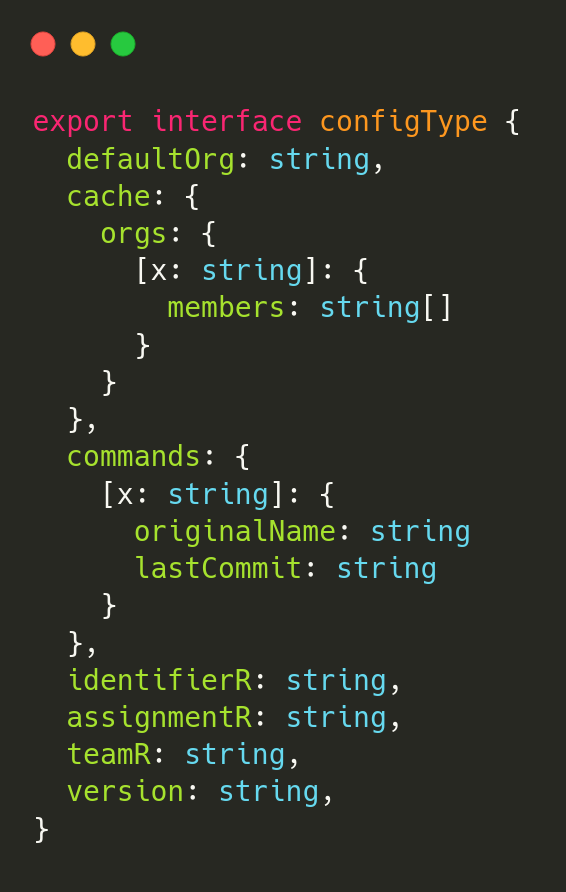
\includegraphics[width=0.5\textwidth]{images/configType.png}}
    \caption{Tipado fuerte en el archivo de datos}
    \label{fig:configType}
\end{figure}

No obstante, TypeScript es un lenguaje compilado y como tal requiere de su propio compilador. 
Esto añadiría otra dependencia al sistema aparte de Node.js. 
Más preocupante aún sería pedirle a nuestro usuario que compilase el código cada vez que vaya a instalar o actualizar.
Hay otras herramientas como \href{https://www.npmjs.com/package/ts-node}{ts-node} que nos permitirían ejecutar el código directamente, pero no solo estamos añadiendo más dependencias, sino que el tiempo de arranque de la aplicación se vería enormemente afectado, incluso si se utiliza un \gls{JIT}(\emph{just-in-time compiler}). 
Para solucionar estos problemas se ha optado por hacer compilación anticipada o \gls{AOT} (ahead-of-time) en cada \emph{commit} que se realice con un hook\cite{hook} de \verb|Git|.

%En el apartado de diseño[TODO añadir referencias] se explica en más detalle los efectos que ha tenido esta estrategia.

En cuanto a dependencia de desarrollo, se ha usado como gestor de paquetes \verb|npm|\cite{npm} por mera preferencia personal.

\subsection{La librería {\tt commander}}
La librería \verb|commander| es muy popular para la creación de aplicaciones \gls{CLI}, se encarga de parsear los argumentos y flags de la línea de comandos, de los mensajes de error relacionados con la creación de dichos argumentos e implementa un sistema de ayuda basándose en las especificaciones establecidas.

Es una parte esencial del ecosistema, a efectos prácticos genera la interfaz mínima necesaria, entre el usuario y el programa y la solución nativa \verb|process.argv| es muy pobre y primitiva en comparación.

Los motivos por los cuales se ha optado específicamente por \verb|commander| son:
\begin{itemize}
    \item \textbf{Popularidad.} Lo cual se traduce en un software a prueba de errores y con abundante documentación.
    \item \textbf{Cero dependencias.} Es bastante remarcable que un paquete del ecosistema de \verb|JS| sea autosuficiente, y nos ayuda en minimizar el tamaño y mantenimiento de nuestro software, en especial en la parte del \verb|core| que interesa que sea lo más convenientemente ligero.
\end{itemize}

\subsection{La librería {\tt shelljs}} \label{shelljs}
La librería {\tt shelljs} es el paquete que me permite llamar a comandos de la terminal desde el código fuente, independientemente del sistema operativo.

Incluye comandos propios de los sistemas Unix como \verb|cp|, \verb|rm| o \verb|which| entre otros, y un comando \verb|exec| para ejecutar cualquier otro comando no contemplado por su API.

Es bastante trivial de usar, pero su interfaz es algo pobre ante todas las posibilidades que ofrece la terminal. Alimentar la \verb|STDIN| con variables del programa, cuando el comando ya ha empezado su ejecución, o mandar una señal de cierre, no es posible al momento de escribir estas líneas. Ha habido intentos de ofrecer una \href{https://github.com/shelljs/shelljs/pull/432}{solución apropiada}, pero no ha habido avances, por lo que se ha tenido que recurrir a soluciones alternativas. Se puede ver una explicación más detallada y el porqué este comportamiento es necesario en el capítulo \textbf{Implementación}, en la sección de \verb|gh-edu-data| (\ref{impl:gh-edu-data}).

\subsection{La librería inquirer}
La librería \verb|inquirer| me permite conseguir datos del usuario de forma interactiva (figura \ref{fig:data-desiredData}). Es una colección de interfaces comunes como:
\begin{itemize}
    \item Confirmación
    \item Múltiple selección (checkbox)
    \item Listas a la \verb|fzf|
\end{itemize}

El método principal para conseguir input del usuario de forma interactiva es \verb|fzf|. La librería \verb|inquirer| carece de  características como la búsqueda difusa o \verb|stdin| dinámico. La utilidad \verb|fzf| es una herramienta diseñada para trabajar con listas.  En aquellas ocasiones que se requiere una simple confirmación o que el usuario tenga que escribir manualmente, se recurre a \verb|inquirer|. 

A pesar de no ser tan potente como \verb|fzf|, \verb|inquirer| es una librería nativa de \verb|JS|, por lo que ha sido más fácil trabajar con ella, especialmente en lo referente al manejo de errores.

\section{El Lenguaje Go} \label{go}
En una de las extensiones se utiliza el lenguaje de programación Go \cite{go}, el motivo de su uso se explica mejor en su respectivo apartado (\ref{diseño:gh-edu-plagiarism}).

Go es un lenguaje relativamente moderno (2009), que ha tenido una aceptación rápida en las tecnologías de la nube, como pueden ser servidores, pero también se ha utilizado mucho en el desarrollo de aplicación de terminal, de hecho, \verb|GitHub CLI| y su predecesor \verb|hub| han sido desarrollados usando Go.

Dentro del ámbito de este proyecto, las ventajas de Go son varias:
\begin{itemize}
    \item \textbf{Binario enlazado estáticamente.} Por lo que los usuarios no tiene que tener instalado \verb|Go|
    \item \textbf{Arranque inmediato.} A medida que las extensiones y el \verb|core| escritos en \verb|JS|/\verb|TypeScript| iban creciendo en tamaño y en dependencias de desarrollo, el rendimiento de la aplicación iba decayendo. Por lo general no es especialmente notorio ni grave, pero donde más se nota es cuando la aplicación empieza la ejecución, principalmente debido a los procesos que se tienen que ejecutar al inicio, como la validación del archivo de datos o la carga de extensiones instaladas.
    \item \textbf{Mejor integración con la terminal.} Los paquetes \href{https://pkg.go.dev/os}{os} e \href{https://pkg.go.dev/io}{io} de la librería estándar han sido de gran ayuda. He podido utilizar todas las características de \verb|fzf| y \verb|jq| manteniendo un código legible y mantenible.
    \item \textbf{Manejo de errores.} El manejo de errores en Go es bastante explícito. Esto hace que el código sea más verboso, pero tengo la seguridad de que mi aplicación tiene todos los posibles errores cubiertos. El usuario no va a ver ningún \emph{stack trace}, a no ser que el mensaje de error este destinado al programador.
\end{itemize}

En cuanto a desventajas, podemos hablar de la distribución:

\begin{itemize}
    \item Go es un lenguaje compilado: a diferencia de TypeScript, no compila a código fuente, sino a código máquina. 
    \item El propio equipo de \verb|gh| proporciona una GitHub Action \cite{githubAction} con nombre \href{https://github.com/cli/gh-extension-precompile}{gh-extension-precompile} que compila el código y lo guarda en el apartado de ``Releases`` de GitHub, a la hora de instalar o actualizar, el comando \verb|gh extension install| que se utiliza de forma interna, descarga el binario para el sistema operativo y arquitectura apropiados. 
    \item Esto ralentiza la productividad al tener que esperar que se compile a todas las plataformas (Linux, Mac OS, Windows) antes de poder probar los resultados con el resto del ecosistema.
\end{itemize}

\begin{figure}[htb]
    \centering
    \makebox[\textwidth][c]{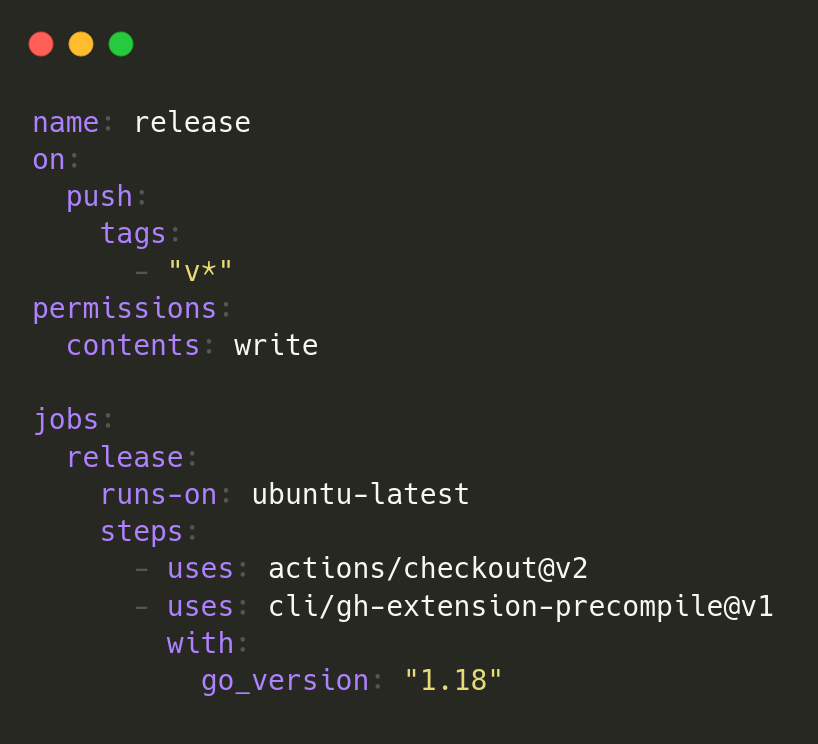
\includegraphics[width=0.5\textwidth]{images/gitHubRelease.png}}
    \caption{Script GitHub release}
    \label{fig:gitHubRelease}
\end{figure}

\subsection{La librería cobra}
La librería cobra \cite{cobra} es para \verb|Go| lo que commander es para javascript: Una librería que permite crear aplicaciones de líneas de comandos no triviales. Generando ayuda automáticamente, autocompletado y con una integración perfecta con viper.

\subsection{La librería viper}
La librerìa
{\tt viper}\cite{viper} es una librería para leer archivos de configuración, en este caso data.json. 
También me permite enlazar datos que se puedan conseguir desde variables de entornos, línea de comandos o archivo de configuración en una sola variable, en ese orden de prioridad.

\section{El Lenguaje jq (JSON Query)}

Para el manejo no trivial de ficheros \verb|JSON| se ha usado el \gls{DSL} jq\cite{jq}, un lenguaje de muy alto nivel que nos permite procesar ficheros \verb|JSON| desde la terminal. 

Si bien es cierto que uno de los motivos para usar \verb|JS| como lenguaje de desarrollo fue la facilidad con la que podemos manejar los ficheros \verb|JSON|, \verb|jq| puede ser más productivo cuando se trabaja en el contexto de la terminal, como es el caso cuando se trabaja con programas como \verb|gh api| o \verb"fzf", que  producen o procesan información en formato JSON a través de los canales o pipelines. 

Procesar JSON con \verb|jq| puede simplificar la tarea de previsualizar información adicional de un \emph{elemento} que está siendo seleccionado. Véase, por ejemplo, la extensión {\tt gh-edu-view} (\ref{sec:gh-edu-view-implementation}).

\section{El Lenguaje \LaTeX{} y Overleaf}
Para la elaboración de este documento se ha usado \LaTeX{}, 
en específico la implementación de \href{https://www.overleaf.com/}{overleaf}\cite{overlife}.
Gracias a esto hemos podido sincronizar con GitHub,
mantener un historial del documento, 
se ha simplificado la instalación de paquetes  y 
tenemos una copia accesible en línea que se sincroniza automáticamente


%%%%%%%%%%%%%%%%%%%%%%%%%%%%%%%%%%%%%%%%%%%%%%%%%%%%%%%%%%%%%%%%%%%%%%%%%%%%%%%
\newpage{\pagestyle{empty}}
\thispagestyle{empty}

\chapter{\LARGE Modo de uso}
\label{chapter:modo-de-uso}

En este capítulo se explica como se utiliza el ecosistema, con intención de que se pueda entender el propósito de cada extensión. En los capítulos siguientes se entrará en más detalle con respecto a la toma de decisiones en el diseño y como se ha logrado implementar todo el ecosistema 

\section{El Núcleo de {\tt gh edu}: Core}

El diseño de la extensión \verb|gh-edu| sigue el \gls{strategy pattern} y consta de un código núcleo (\verb|core|) que coordina las estrategias y extensiones. Algunas de las estrategias más básicas forman parte del código núcleo que se provee con la \verb|gh-extension| \verb|gh-edu|.

Todos los comandos de \verb|gh-edu|  se pueden ejecutar desde la línea de comandos y cuando es apropiado cuentan con un modo interactivo. La figura \ref{fig:ghEduHelp} muestra los subcomandos disponibles en el núcleo.

\begin{figure}[h]
    \centering
    \makebox[\textwidth][c]{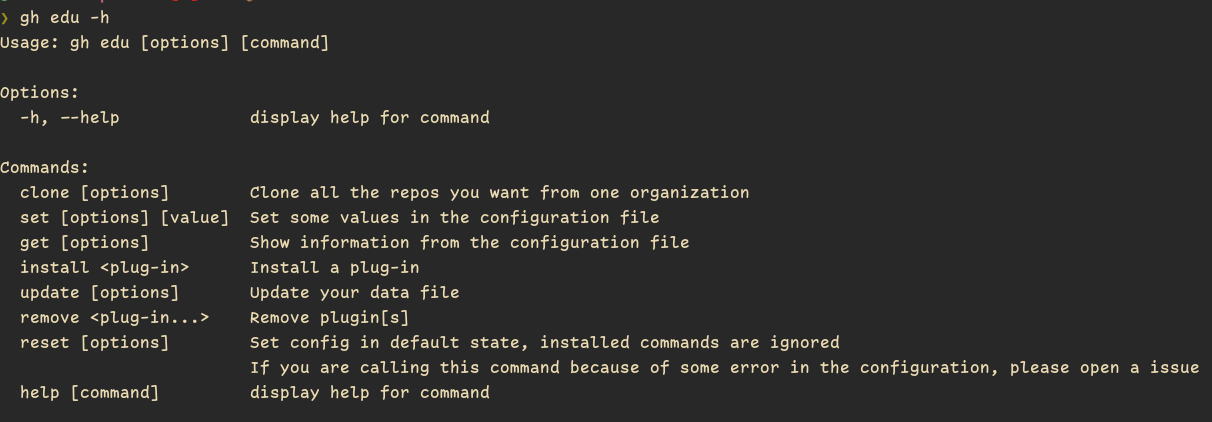
\includegraphics[width=\textwidth]{images/gh-edu-help.png}}
    \caption{Ayuda general de gh edu}
    \label{fig:ghEduHelp}
\end{figure}

Para este apartado es relevante saber que \verb|gh-edu| trabaja en torno a un archivo de datos o registro llamado \verb|data.json|.

Este archivo de datos guarda información
\begin{itemize}
    \item de las extensiones instaladas 
    \item de la versión y configuración de las extensiones instaladas,
    \item de información proveida por las extensiones a solicitud del usuario
    \item del usuario y de la configuración del usuario 
    \item del estado actual del sistema \verb|gh-edu| (por ejemplo, cuál es la organización GitHub por defecto)
    \item de datos obtenidos desde la API de GitHub y que han sido cacheados
\end{itemize}
 este fichero se guarda de forma persistente en \verb|$HOME/.config/gh-edu/data.json|. Este directorio esta siempre bajo control de versiones y puede estar enlazado a un remoto llamado \verb|https://github.com/github-user:/gh-edu-profile|.

Dicho fichero es único y privado para cada usuario y se obtiene de una de estas dos formas:
\begin{itemize}
    \item Se crea uno nuevo a partir de una plantilla base, la cual tiene los elementos mínimos para dar el fichero por válido, o 
    \item Se descarga automáticamente si el usuario tiene uno propio dentro de un repositorio en GitHub en su cuenta con el nombre \verb|<github-user>/gh-edu-profile|. 
\end{itemize}

Se entrará más en detalle sobre \verb|data.json| en el capítulo \textbf{Diseño} \ref{diseño:data}.

\subsection{Subcomando set}
Comando importante, utilizado para establecer la configuración en el fichero de datos
\begin{figure}[h]
    \centering
    \makebox[\textwidth][c]{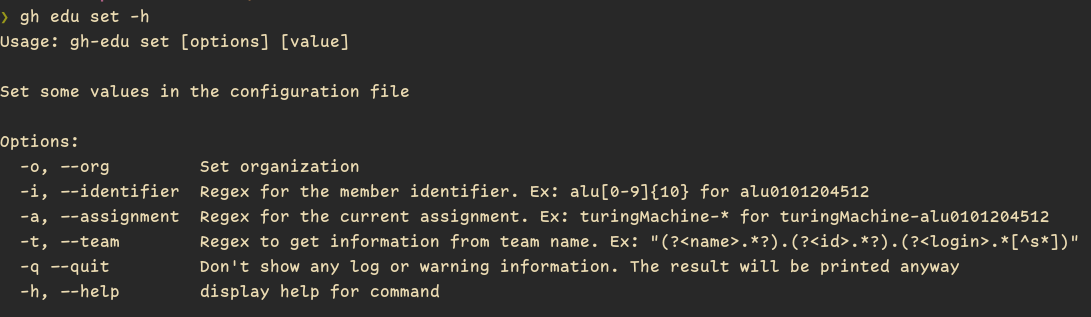
\includegraphics[width=\textwidth]{images/set-help.png}}
    \caption{Ayuda de gh edu set}
    \label{fig:ghEduSetHelp}
\end{figure}

\begin{itemize}
    \item \textbf{-o, -{}-org.} Específica la organización con la que estamos trabajando actualmente. En la mayoría de universidades, las organizaciones de GitHub suelen estar asociados a las asignaturas.
    Ejemplo de uso: \verb|gh edu set -o gh-cli-for-education|, si pertenecemos a la organización se registrará como organización actual y se guardará como cache a los miembros pertenecientes de la organización.
    Si no se le pasa un valor, se activará \verb|fzf| para poder elegir entre las organizaciones a las que el usuario pertenezca.
    \item \textbf{-q, -{}-quiet.} No se muestra ninguna información por pantalla, más allá del resultado y los errores.
    \item \textbf{-i, -{}-identifier.} Expresión regular para identificar los identificadores de los alumnos, en el caso de la ULL utilizamos \verb|alu| seguido de 10 números del 0 al 9. que se corresponde con la expresión regular \verb|alu[0-9]\{10\}|
    \item \textbf{-t, -{}-team.} Expresión regular para poder extraer información del nombre de los equipos. Está pensada para que se utilice con agrupamientos con nombre (``named captured group``). Por ejemplo, la expresión regular:\\ \verb|(?<name>.*?).(?<id>.*?).(?<login>.*[^s*])|\\
    Aplicada sobre el siguiente nombre de equipo:\\
    \verb|cristo-garcia-gonzález.alu0101204512.ggcristo|\\
    Es capaz de generar automáticamente la siguiente información:
    \begin{itemize}
        \item \textbf{name:} cristo-garcia-gonzález
        \item \textbf{id:} alu0101204512
        \item \textbf{login:} ggcristo
    \end{itemize}
    \item \textbf{-a, -{}-assignment}. Expresión regular para marcar los repositorios sobre los que se quiere trabajar. Normalmente, se le asigna un repositorio a cada alumno por asignación/tarea. Por ejemplo: \verb|turingMachine-.*| en el caso de que los repositorios empiecen por \verb|turingMachine| como podría ser \verb|turingMachine-alu0101204512|.
\end{itemize}
El uso que se les dé a estos campos depende deliberadamente de cada desarrollador y profesor.

\subsection{El subcomando core {\tt get}}
\begin{figure}
    \centering
    \makebox[\textwidth][c]{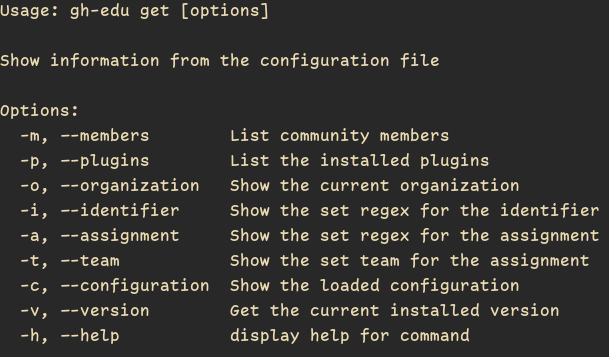
\includegraphics[width=\textwidth]{images/get-help.png}}
    \caption{Ayuda de gh edu get}
    \label{fig:ghEduGetHelp}
\end{figure}
El comando \verb|get| muestra la información que se tiene actualmente
\begin{itemize}
    \item \textbf{-m, -{}-members.} Muestra los miembros de la organización establecida. Lee de la caché, si es posible.
    \item \textbf{-p, -{}-plugins.} Lista las extensiones y comandos disponibles tanto los que vienen con el core (builtin) como los instalados por el usuario.
    \item \textbf{-o, -{}-org.} Muestra la organización marcada.
    \item \textbf{-i, -{}-identifier}. Muestra la expresión regular establecida para detectar los identificadore de los alumnos.
    \item \textbf{-a, -{}-assignment.} Muestra la expresión regular establecida para filtrar los repositorios deseados.
    \item \textbf{-t, -{}-team.} Muestra la expresión regular establecida para recolectar información de los nombres de los equipos.
    \item \textbf{-v, -{}-version.} Muestra la versión instalada.
    \item \textbf{-c, -{}-configuration.} Muestra por pantalla la toda la configuración y datos cargados.
\end{itemize}

\subsection{El subcomando core {\tt clone}}
El comando \verb|clone| solo tiene dos opciones \verb|--org| por si queremos clonar de una organización en concreto sin tener que cambiar la organización establecida y \verb|--quiet| para solo mostrar los mensajes de errores (y \verb|--help|).
Este comando fue planeado para clonar varios repositorios en paralelo usando la librería \href{https://www.npmjs.com/package/concurrently}{concurrently}

\begin{figure}[H]
    \centering
    \makebox[\textwidth][c]{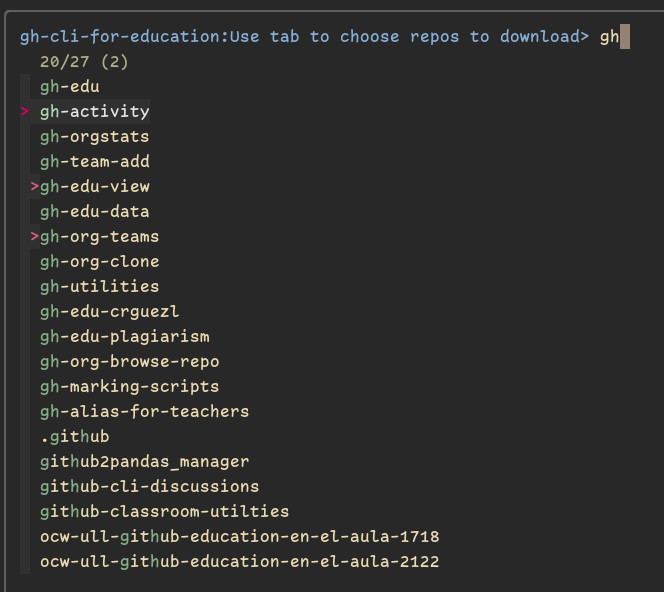
\includegraphics[width=\textwidth]{images/clone.png}}
    \caption{clone usando fzf}
    \label{fig:clone}
\end{figure}

En la figura \ref{fig:clone} se ve la interfaz de \verb|clone| con \verb|fzf|, arriba a la izquierda aparece el nombre de la organización y podemos seleccionar múltiples repositorios presionando \emph{TAB} y filtrarlos de forma difusa (nótese como \verb|.github|, el cual no es una coincidencia exacta, aparece en la lista), para aceptar se pulsa \emph{ENTER}.

\subsection{El subcomando {\tt install}}
Como su nombre indica \verb|install| instala extensiones añadiendo más comandos al sistema. No acepta otro argumento más que el nombre de la extensión que queremos instalar y solamente tiene el \verb|flag| \verb|--quiet|, con la misma funcionalidad que el resto de extensiones.

El código de las extensiones tiene que estar alojado en GitHub y solo funciona con la rama por defecto.

El comando se ejecuta de la siguiente forma:\\
\verb|gh edu install <organización/nombre_extension>|

Ejemplo:

\begin{verbatim}
        gh edu install crguezl/gh-edu-browse
        Installing crguezl/gh-edu-browse ...
        Plugin installed in system
        Setting up configuration...
        crguezl/gh-edu-browse installed as browse
\end{verbatim}
Pero si la extensión es \emph{first-party}, es decir, pertenece a la organización \verb|gh-cli-for-education|, no es necesario especificar la organización. Por ende:\\
\verb|gh edu install gh-cli-for-education/view|, es equivalente a \verb|gh edu install view|

\subsection{El subcomando {\tt remove}}
Elimina las extensiones instaladas por el comando \verb|install|. No puede eliminar los comandos \emph{bultin}.\\
El comando se ejecuta de la siguiente forma:\\
\verb|gh edu remove <nombre_extension1> <nombre_extension2> ... <nombre_extensionN>|

\subsection{El subcomando {\tt update}}

\begin{figure}[htb]
    \centering
    \makebox[\textwidth][c]{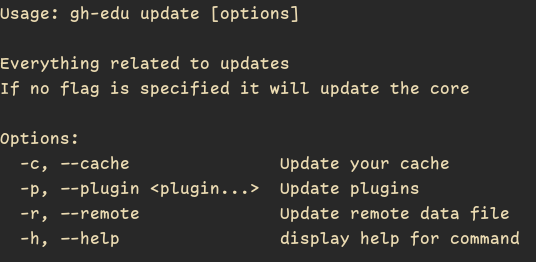
\includegraphics[width=\textwidth]{images/updateHelp.png}}
    \caption{Ayuda de get update}
    \label{fig:updateHelp}
\end{figure}

El subcomando \verb|update| se encarga de todo lo relacionado con las actualizaciones.
\begin{itemize}
    \item \textbf{-c, -{}-cache.} Actualiza todos los valores posibles de la caché. No es un comando esencial, especialmente cuando algunos comandos ya actualizan ciertas partes de la caché, pero es recomendable correrlo desde que se obtenga el fichero de datos data.json.
    \item \textbf{-p, -{}-plugin.} Actualiza una o varías extensiones. Si no tiene un argumento, actualiza todas las extensiones instaladas.
    \item \textbf{-r -{}-remote.} Actualiza el repositorio gh-edu-profile con los datos locales. En caso de no existir se le pregunta al usuario si quiere crear dicho repositorio.
    \item \textbf{Sin argumentos ni \emph{flags}.} Si el usuario ejecuta el comando sin argumentos, el propio \verb|core| se actualizará. Es equivalente a \verb|gh extension upgrade gh-edu|. Fue creado para mantener la simetría con el resto de comandos.
\end{itemize}

\subsection{El subcomando {\tt reset}}
Restaura la configuración a su estado original dejando intacto la información sobre los comandos instalados, si también se desea borrar dicha información se puede usar el flag \verb|--force|, aunque no es recomendable, ya que generaría una incongruencia con las extensiones que están realmente instaladas en el sistema y la propia información del sistema.

Este comando existe por meros motivos de depuración y en caso de que un error en la implementación del sistema lleve al usuario a un estado anormal. No se debe de usar con regularidad.

\section{La Extensión {\tt view}}
Es una pequeña extensión para mostrar información relevante sobre la organización, por lo que es necesario tener una organización establecida.

Dentro del contexto del TFG se ha desarrollado un único comando \verb|members| que muestra información sobre los miembros de la organización. Se espera ampliarlo para que también muestre otro tipo de información que pueda ser relevante al profesorado y alumnado (vease \ref{conclusion}).

Esta extensión también aprovecha la expresión regular del identificador guardado en data.json para intentar conseguir los identificadores de los alumnos leyendo varios campos en su cuenta de GitHub

Se puede ejecutar directamente como: \verb|gh edu view members| o añadir el flag \verb|--id| para usar un identificador que tendrá prioridad sobre el establecido en \verb|data|.
\begin{figure}[H]
    \centering
    \makebox[\textwidth][c]{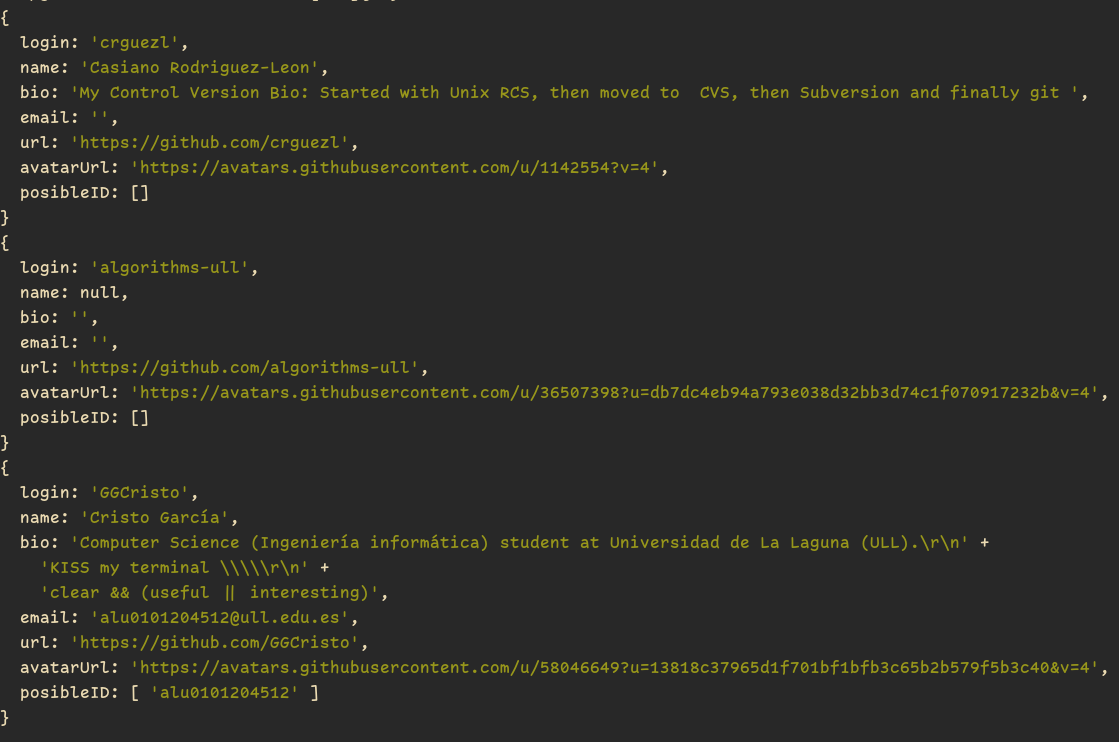
\includegraphics[width=\textwidth]{images/view.png}}
    \caption{Ejemplo de uso de gh view con --id ``alu[0-9]\{10\}``}
    \label{fig:view}
\end{figure}

\section{La Extensión {\tt data}}

Ha sido creado para manejar y guardar información variada de los alumnos.

Para instalarla:
\begin{verbatim}
    gh edu install data
\end{verbatim}

Tiene tres comandos principales: \verb|log|, \verb|teams| y \verb|team-add|:


\begin{verbatim}
    $ gh edu data -h
    Usage: gh-edu-data [options] [command]
    
    Options:
      -h, --help                 display help for command
    
    Commands:
      log [options] <inputFile>  Get relevant information about you students
      teams [options]            Get relevant information about you students using
                                 teams
      team-add [options]         Create teams with certain patterns to get
                                 information later on. Empty spaces will become '-'
      help [command]             display help for command
\end{verbatim}

\subsection{El subcomando {\tt log}}
El objetivo de \verb|log| es principalmente relacionar la cuenta institucional de un alumno con su cuenta de GitHub y conseguir información extra que le pueda ser de utilidad al profesor.

\begin{verbatim}
    gh edu data log -h
    Usage: gh-edu-data log [options] <inputFile>
    
    Get relevant information about you students
    
    Options:
      -o, --output <outputFile>  File to write the resulting data. If not specified
                                 it will write the result to the standard output
      -c, --cache                Cache the information in the configuration file
      -q, --quiet                Don't show any output, except errors
      -h, --help                 display help for command
\end{verbatim}
Se necesita de un fichero inicial con información que el profesor tenga de los alumnos. Dicho fichero de entrada tiene que ser de tipo \verb|JSON|, con un \emph{array} donde cada elemento guarde información de los alumnos. Esta información tiene que contener mínimamente el nombre del alumno, aunque lo apropiado es que contenga el nombre y un identificador. Puede tener más datos (figura \ref{fig:inputJSON}).

Una vez ejecutado el comando, el profesor decide que campos quiere tener de cada alumno (figura \ref{fig:data-desiredData}). Y cuáles de los campos entrantes corresponden al nombre, y en caso de haberlo el identificador (figura \ref{fig:linkFields}). Después, uno a uno y aprovechando la eficaz interfaz de \verb|fzf| y la previsualización de los datos remotos del alumno, se filtra el alumno en cuestión (figura \ref{fig:interface-log}).

Como resultado se obtiene un nuevo fichero JSON que contiene la información dada inicialmente por el profesor, combinada con los datos proporcionados por GitHub (figura \ref{fig:result-log}).

\begin{figure}[H]
    \centering
    \makebox[\textwidth][c]{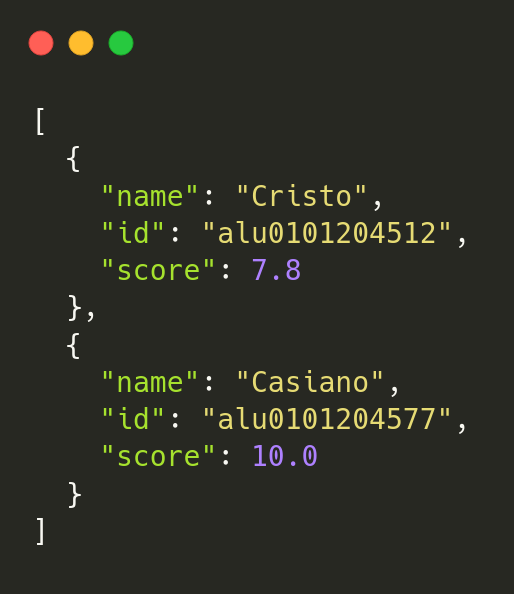
\includegraphics[width=0.5\textwidth]{images/inputJSON.png}}
    \caption{gh edu data log. Ejemplo de archivo de entrada}
    \label{fig:inputJSON}
\end{figure}

\begin{figure}[H]
    \centering
    \makebox[\textwidth][c]{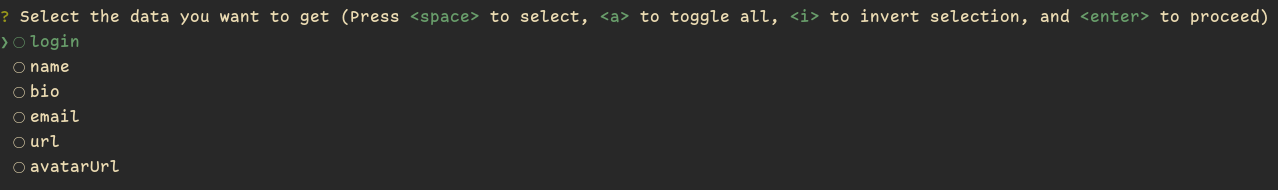
\includegraphics[width=\textwidth]{images/data-select-desiredField.png}}
    \caption{gh edu data log. Seleccionando los datos deseados}
    \label{fig:data-desiredData}
\end{figure}

\begin{figure}[H]
    \centering
    \makebox[\textwidth][c]{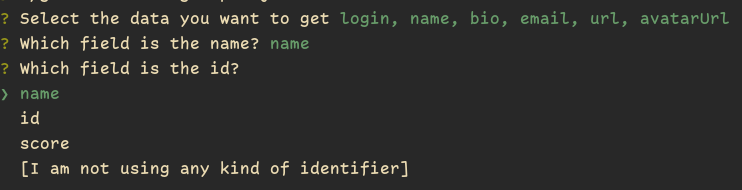
\includegraphics[width=\textwidth]{images/selectFields.png}}
    \caption{gh edu data log. Enlazando los campos del fichero de entrada con el nombre y el ID}
    \label{fig:linkFields}
\end{figure}

\begin{figure}[H]
    \centering
    \makebox[\textwidth][c]{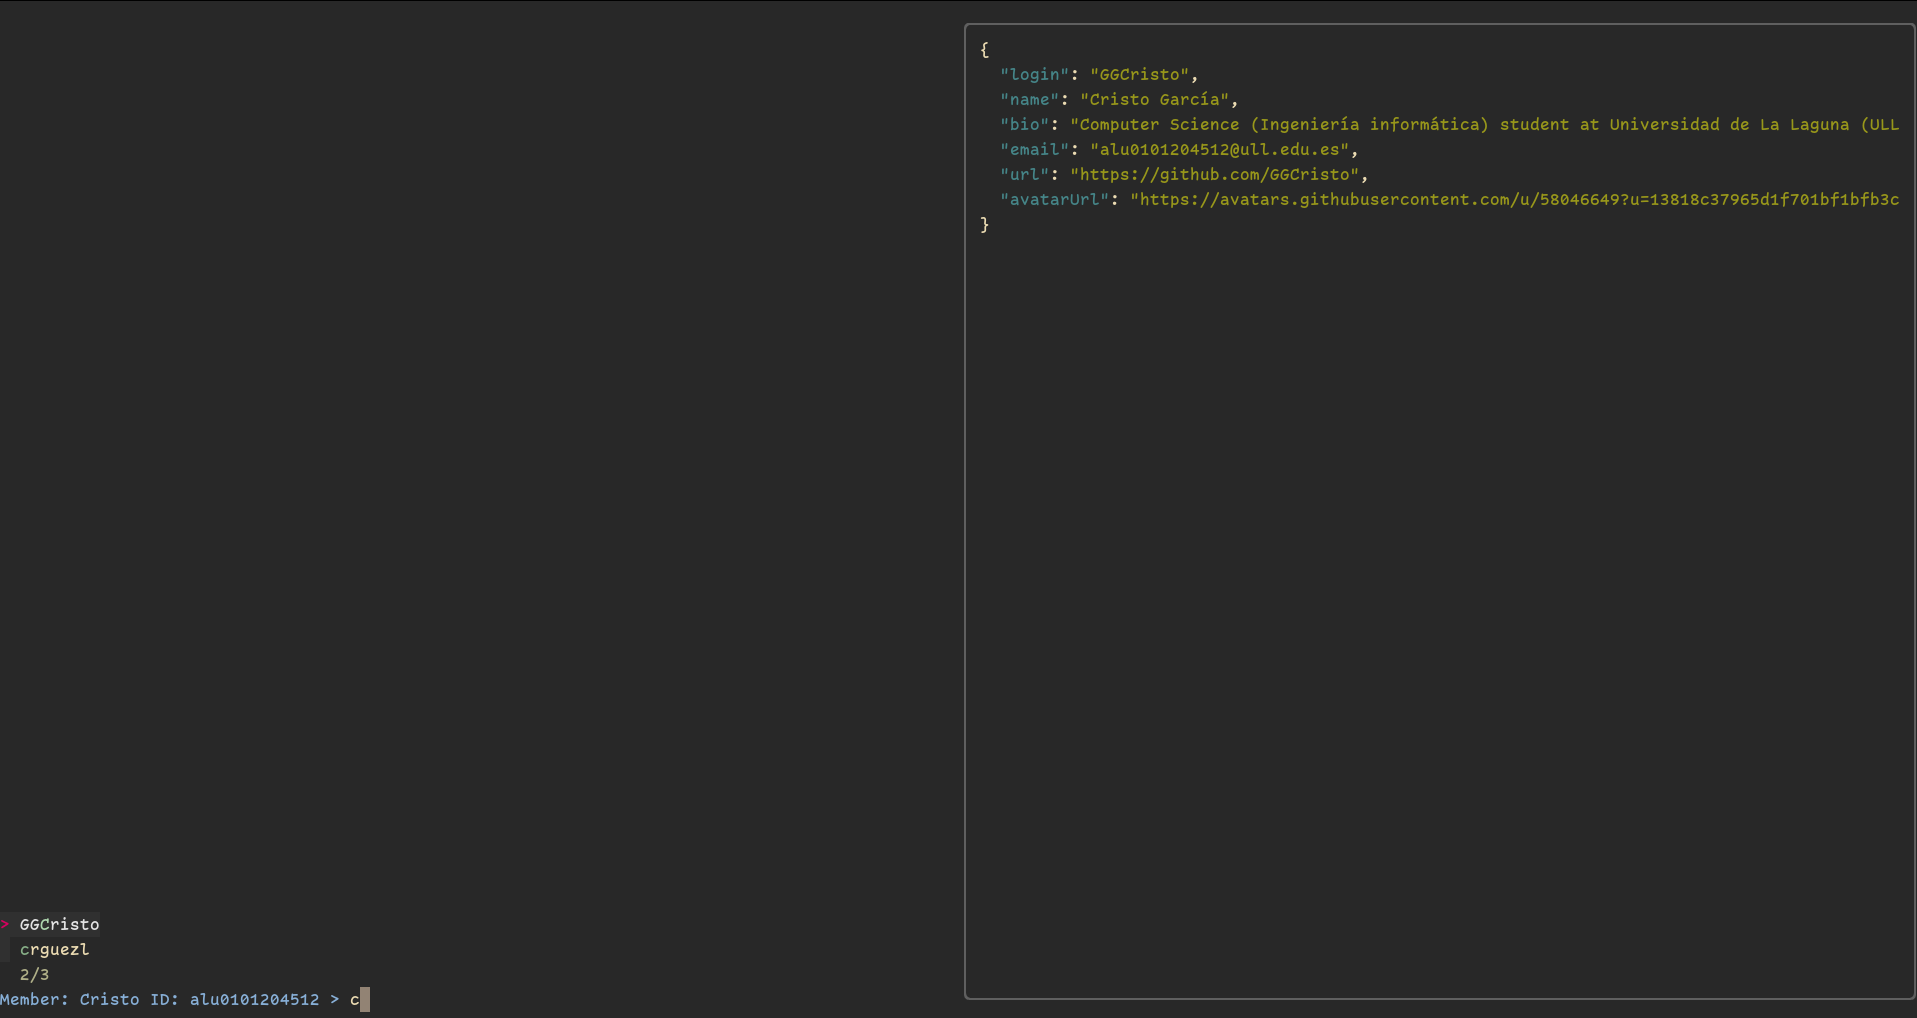
\includegraphics[width=\textwidth]{images/interface-log.png}}
    \caption{gh edu data log. Interfaz principal}
    \label{fig:interface-log}
\end{figure}

\begin{figure}[H]
    \centering
    \makebox[\textwidth][c]{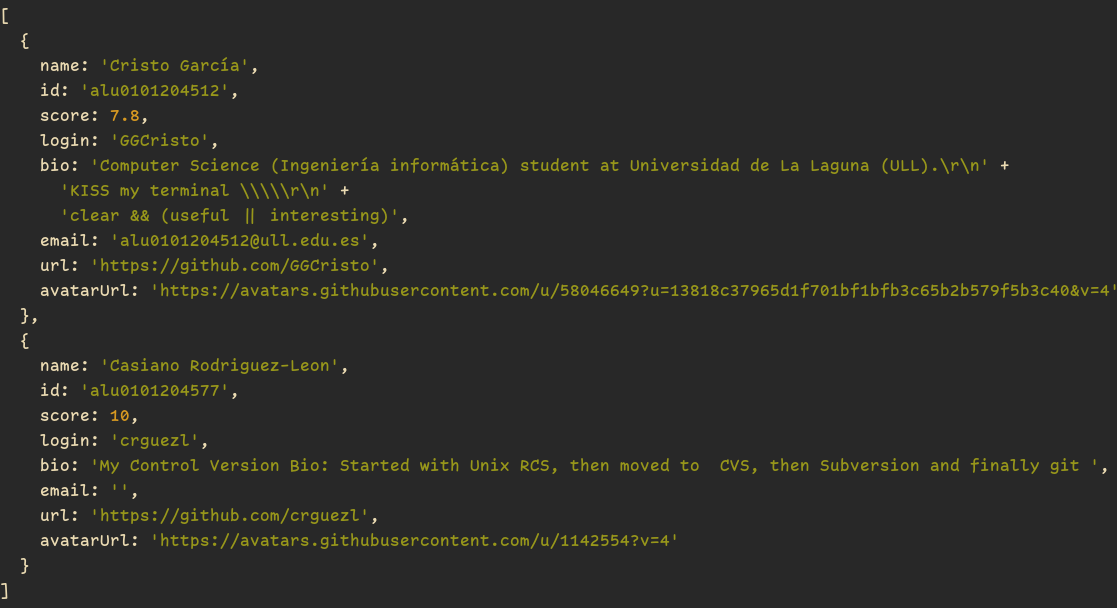
\includegraphics[width=\textwidth]{images/result-log.png}}
    \caption{gh edu data log. Resultado}
    \label{fig:result-log}
\end{figure}

Tiene los siguientes \verb|flags| para modificar su comportamiento:
\begin{figure}[H]
    \centering
    \makebox[\textwidth][c]{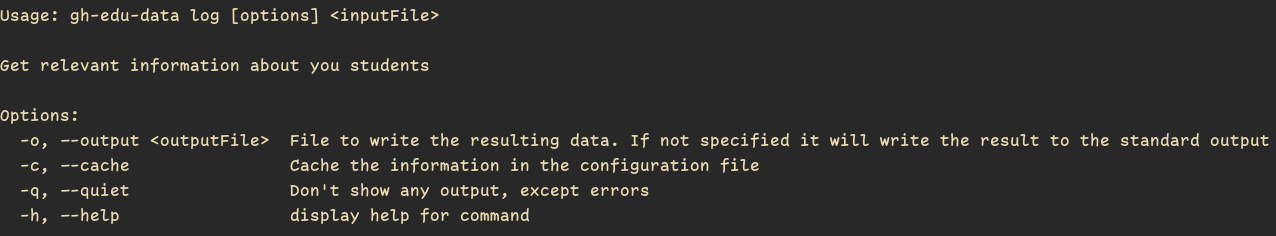
\includegraphics[width=\textwidth]{images/data-log-help.png}}
    \caption{gh edu data log. Ayuda}
    \label{fig:data-log-help}
\end{figure}

Estos \verb|flags| se comportan igual que en el resto de subcomandos, a excepción de \textbf{c, -{}-cache}, en cuyo caso, estamos indicando de que queremos guardar el resultado en una \gls{cache} en el fichero data.json. Un ejemplo del resultado se puede ver en la figura \ref{fig:data}

\subsection{El subcomando {\tt teams}}
Una de las estrategias que suelen utilizar los profesores para tener identificados a los alumnos es que en la primera práctica de la asignatura se procede a crear una asignación de GH Classroom de este modo:
\begin{enumerate}
    \item Usando una asignación de GH Classroom crear una tarea de equipo
    \item Los equipos serán individuales formados por un solo alumno
    \item Cada alumno cuando acepta la asignación crea su equipo le debe dar el nombre según las instrucciones que le haya dado el profesor
\end{enumerate}

Un ejemplo de tal instrucción del profesor sobre el nombre del equipo podría ser: 

"El nombre del equipo debe estar formado por el nombre y apellidos del alumno separado por guiones, seguido del identificador de la universidad. No use tildes ni caracteres especiales".

Por ejemplo para un. alumno dela ULL podría ser algo como \verb|cristo-garcia-gonzalez-alu0101204512|. 

El comando viene gobernado por la expresión regular con paréntesis con nombre 
especificada en la entrada \verb|teamR| del fichero de configuración:
\begin{verbatim}
➜  gh-edu-data git:(casiano) ✗ gh edu get -c | jq '.teamR'
"(?<name>.+)[-_](?<id>.+)"
➜  gh-edu-data git:(casiano) ✗ gh edu get -t
(?<name>.+)[-_](?<id>.+)
\end{verbatim}
Esta expresión regular permite decidir que \verb|name| es la primera parte \verb|cristo-garcia-gonzalez| y que \verb|id| es \verb|alu0101204512|.

\verb|teams| es un comando que tiene el mismo objetivo que \verb|log|, pero se aprovecha de esta estrategia, para que la obtención y búsqueda de dicha información sea inmediata.

El comando actúa sobre la organización por defecto. 
Supongamos fijada la organización de una cierta clase:

\begin{verbatim}
➜  gh-edu-data git:(casiano) ✗ gh edu get -o
ULL-ESIT-PL-2122
\end{verbatim}

El comando tiene las siguientes opciones:

\begin{verbatim}
➜  gh-edu-data git:(casiano) ✗ gh edu data teams -h
Usage: gh-edu-data teams [options]

Get relevant information about you students using teams

Options:
  -o, --output <outputFile>  File to write the resulting data. If not specified
                             it will write the result to the standard output
  -c, --cache                Cache the information in the configuration file
  -q, --quiet                Don't show any output, except errors
  -h, --help                 display help for command
\end{verbatim}

Entonces cuando se ejecuta:

\begin{verbatim}
➜  gh-edu-data git:(casiano) ✗ gh edu data teams
\end{verbatim}

Se conecta a la API de GH para obtener los equipos de un solo miembro he intenta obtener del nombre y propiedades de los equipos de un solo miembro la información necesaria.

Saldrá por stderr mensajes de advertencia para los equipos con mas de un miembro, como este::

\begin{verbatim}
➜  gh-edu-data git:(casiano) ✗ gh edu data teams
Warning! Teams with several members not included in the identification process: {
  "casiano-rodriguez-leon-crguezl": [
    "https://github.com/crguezl",
    "https://github.com/algorithms-ull"
  ]
}
\end{verbatim}

y por stdout saldrá algo como esto:

\begin{verbatim}
[
  {
    "url": "https://github.com/AdalDiazFarina",
    "email": "",
    "nameInGH": "Adal Díaz Fariña",
    "name": "adal-diaz-fariña",
    "id": "alu0101112251"
  },
  ... etc.
  {
    "url": "https://github.com/CorEHarD5",
    "email": "sergiodlbg@gmail.com",
    "nameInGH": "alu0100953275",
    "name": "sergio-barrera-garcia",
    "id": "alu0100953275"
  }
]
\end{verbatim}

\subsection{El subcomando {\tt team-add}}
Este subcomando fue creado como respuesta al subcomando \verb|teams| con la intención de también facilitar el trabajo a los alumnos, a la hora de crear los equipos en la organización.

Se aprovecha del campo \verb|teamR| para saber que datos pedirle al alumno. Por ejemplo, si se tiene en \verb|teamR| el siguiente valor \verb|(?<name>.*?)\.(?<id>.*?)\.(?<age>.*[^s*])|. El programa le preguntará al alumno por \verb|name|, \verb|id| y \verb|age|. Y creará un equipo en la organización especificada por \verb|defaultOrg|, con dichos datos y el alumno como miembro.

\begin{figure}[H]
    \centering
    \makebox[\textwidth][c]{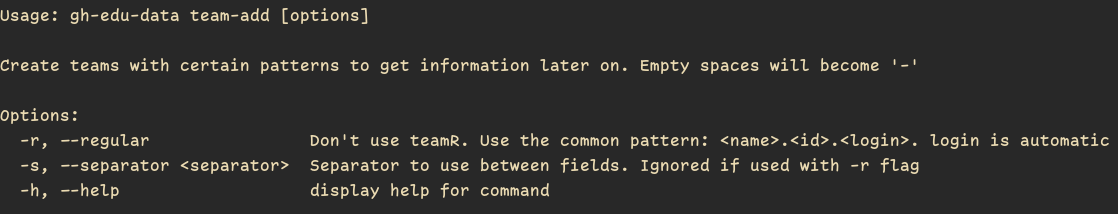
\includegraphics[width=\textwidth]{images/team-add-help.png}}
    \caption{Ayuda para subcomando team-add}
    \label{fig:team-addHelp}
\end{figure}

\begin{itemize}
    \item \textbf{-r, -{}-regular.} Ignora el campo \verb|teamR| y el flag \textbf{-s, -{}-separator}. Le pregunta al alumno por su nombre e identificador y crea un equipo con dicha información, más su identificación en GitHub. El separador es \lq.\rq. Se ha considerado que este patrón es lo suficientemente conveniente, para justificar un \verb|flag| exclusivo para él.
    \item \textbf{-s, -{}-selector.} No se ha encontrado una manera fiable de deducir el selector a partir de \verb|teamR|, por lo que el alumno tendrá que especificarlo con este \verb|flag|. Si se omite, el programa le preguntará al usuario de forma interactiva.
\end{itemize}

\section{La Extensión {\tt plagiarism}}
Es una extensión para detectar el porcentaje de similitud en las tareas de los alumnos. Se puede usar principalmente para ayudar al profesor a detectar plagio.

Genera un grafo mostrando los porcentajes y el número de líneas que son similares entre cada par de alumnos, y un informe con un enlace para ver las similitudes del código fuente.\\
Es necesario tener instalados varías dependencias:
\begin{enumerate}
    \item \textbf{MOSS (Measure Of Software Similarity)\cite{MOSS} script.} El usuario tiene que solicitar un fichero en el que viene incluido la \emph{key}/\emph{id} correspondiente. Los pasos del proceso están en su \href{https://theory.stanford.edu/~aiken/moss/}{página web}.
    \item \textbf{Perl.} Para poder ejecutar el script de \verb|MOSS|.
    \item \textbf{mossum\cite{mossum}.} Para generar el grafo con los datos de \verb|MOSS|.
\end{enumerate}
\verb|fzf| es opcional
\begin{figure}[H]
    \centering
    \makebox[\textwidth][c]{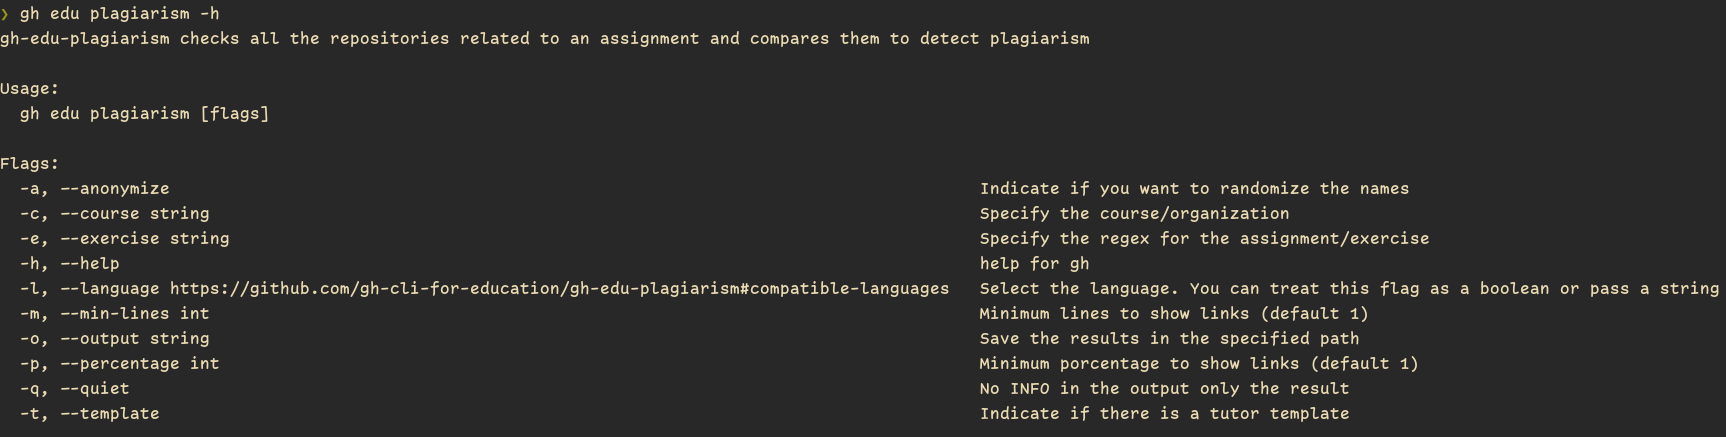
\includegraphics[width=\textwidth]{images/plagiarism-help.png}}
    \caption{Ayuda de gh edu plagiarism}
    \label{fig:plagiarismHelp}
\end{figure}

\begin{itemize}
    \item \textbf{-a, -{}-anonymize}, muestra el grafo con nombres falsos aleatorios. Se podría usar en caso de que el profesor quiera mostrar el grafo a la clase.\\
    \emph{Nota: Este comando solo se aplica al grafo, el informe se queda intacto, ya que está destinado a ser consumido únicamente por el profesor}
    \item \textbf{-c, -{}-course <course>}. La organización se puede indicar con este flag, y toma prioridad con respecto al archivo de configuración.
    \item \textbf{-e, -{}-exercise <exercise>}. La expresión regular para la tarea se puede indicar con este flag, y toma prioridad con respecto al archivo de configuración.
    \item \textbf{-l, -{}-language <language>}. Indica el lenguaje de programación utilizado.\\
    A pesar de que esta sea un campo obligatorio para que funcione el programa, si se omite se pedirá más tarde de forma interactiva con \verb|fzf|
    
    Se aceptan los mismos lenguajes que \verb|MOSS| acepta, los cuales son: c, cc (C++), java, ml (Meta Language), pascal, ada, lisp, scheme, haskell, fortran, ascii, vhdl, perl, matlab, python, mips, prolog, spice, vb (Visual Basic), csharp (C\#), modula2, a8086 (8086 assembly), javascript, plsql (PL/SQL), verilog.
    \item \textbf{-m, --min-lines <lines> (Por defecto: 1)}. Indica cuál es el número mínimo de líneas que deben ser similares para que el estudiante salga en el grafo.
    \item \textbf{-o, --output <path>}. Indica donde se quiere guardar el resultado. El informe y el grafo se guardan en el directorio temporal del sistema hasta la siguiente ejecución, utilizando este flag se puede indicar donde guardar los resultados de forma persistente.
    \item \textbf{-p, -{}-percentage <percentage>(Por defecto: 1)}. Indica cuál es el porcentaje mínimo de similitud entre los pares para mostrar en el grafo.
    \item \textbf{-q, -{}-quiet}. No se muestra ninguna información, aparte del informe final. Útil para redirigir el informe a otro fichero.
\end{itemize}
%%%%%%%%%%%%%%%%%%%%%%%%%%%%%%%%%%%%%%%%%%%%%%%%%%%%%%%%%%%%%%%%%%%%%%%%%%%%%%%
\newpage{\pagestyle{empty}}
\thispagestyle{empty}

\chapter{\LARGE Diseño}
\label{chapter:tres}

En este capítulo se explica el porqué se han tomado ciertas decisiones, problemas y dudas que han ido surgiendo a lo largo del desarrollo y se muestra las especificaciones del sistema.

\section{Consideraciones de Diseño}
Cuando se utiliza GitHub en el ámbito académico no hay una sola forma de organizar las clases y queda a criterio de cada profesor. Es por esto que una aplicación \emph{opinionated} o inflexible no puede llegar muy lejos. Como resultado, se ha decidido crear un sistema modulable y extendible a través de extensiones, con la aplicación principal manejando información que pueda resultar útil para cualquier extensión futura, pero que sea lo más genérica posible. Esta plasticidad se intenta conseguir mediante la configuración y las extensiones. Por eso se permite en un buen número de puntos  de la configuración , la existencia de campos vacíos y que algunos de estos sean expresiones regulares. De esta forma, diferentes extensiones, pueden utilizar diferentes estrategias y utilizar los datos disponibles como se crea conveniente, haciendo que cada profesor pueda utilizar el programa sin que su metodología de trabajo se vea condicionada.

También tenemos que tener en cuenta que nuestro público objetivo son profesores y alumnos de ingeniería, programación, estadística y relacionados, que utilizan GitHub y que, por lo tanto, tendrán cierto grado de conocimiento con las tecnologías informáticas y la terminal. A su vez, no todas las aplicaciones se van a ver beneficiadas de tener una interfaz gráfica en el navegador y queremos complementar a \verb|GitHub Classroom|, no sustituirlo, por lo que construir el ecosistema en la terminal es la mejor opción.

Las extensiones se subirán a la plataforma de GitHub con el prefijo \verb|gh-edu-|. Se ha elegido tener un \gls{namespace} o prefijo, para diferenciar las extensiones de aquellas extensiones de \verb|gh| que no estén creadas con fines docentes o no tengan intención de aprovecharse del ecosistema.

En un intento de mantener que el ecosistema no sea más complicado de lo necesario, especialmente la interfaz, las peticiones a la \verb|API| de GitHub solo funcionaran con la rama por defecto.

\section{El Núcleo de {\tt gh-edu}}
Construir sobre \verb|gh extension| comandos homónimos como \verb|install| o \verb|remove|, ha sido importante para evitar la reimplementación de un gestor de extensiones desde cero, lo cual hubiese sido excesivo cuando solo se busca tener un mayor control sobre el estado del sistema. También gracias a esto, los creadores de extensiones pueden crear las extensiones en el lenguaje que crean convenientes. Si se trata de un lenguaje interpretado, será suficiente con tener un script escrito en \verb|bash| con el mismo nombre que el del repositorio de GitHub, que se encargue de ejecutar el fichero principal. Para lenguajes compilados es necesario subir los binarios correspondientes al apartado de \verb|Releases| del repositorio y el comando \verb|gh extension install| que se ejecuta internamente se encargará de descargarlo.

\begin{figure}[H]
    \centering
    \makebox[\textwidth][c]{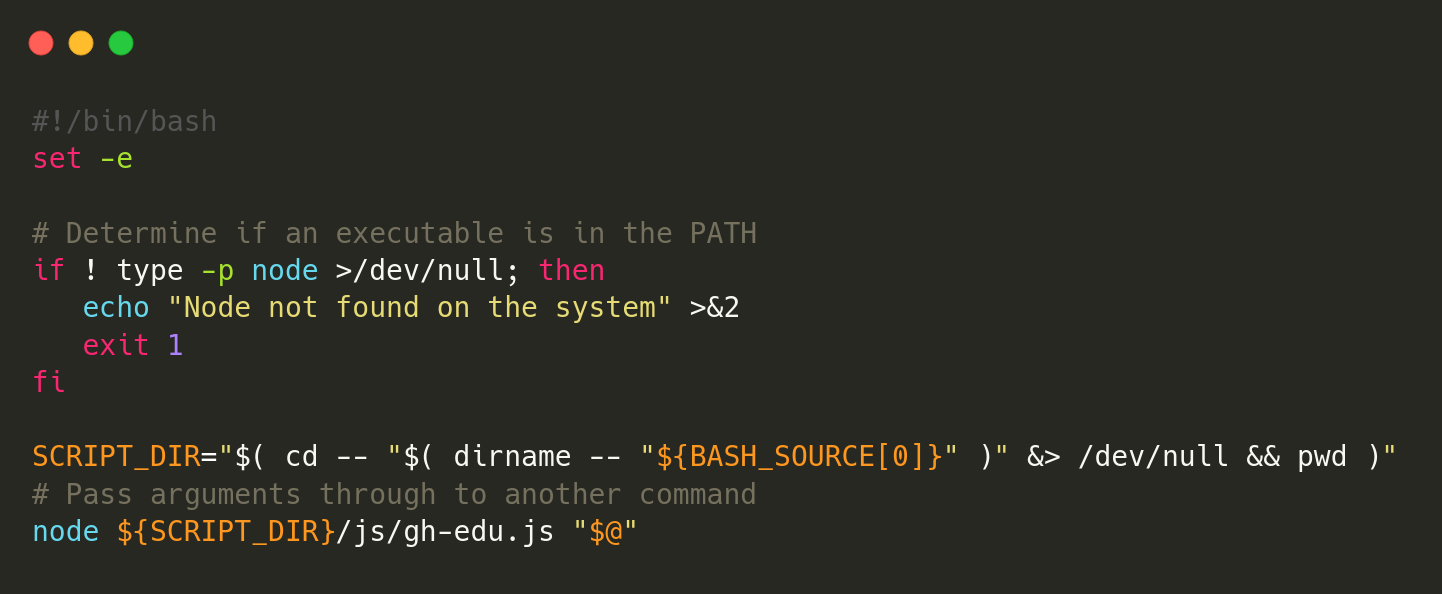
\includegraphics[width=\textwidth]{images/bash.png}}
    \caption{Diseño. Ejemplo de un script para ejecutar una extensión creada con lenguaje interpretado}
    \label{fig:bash}
\end{figure}

\begin{figure}[H]
    \centering
    \makebox[\textwidth][c]{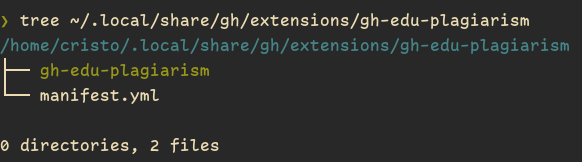
\includegraphics[width=\textwidth]{images/binary.png}}
    \caption{Diseño. Ejemplo de contenido de una extensión creada con lenguaje compilado}
    \label{fig:binario}
\end{figure}

\subsection{El fichero de Configuración {\tt data.json}} \label{diseño:data}

\begin{figure}[H]
    \centering
    \makebox[\textwidth][c]{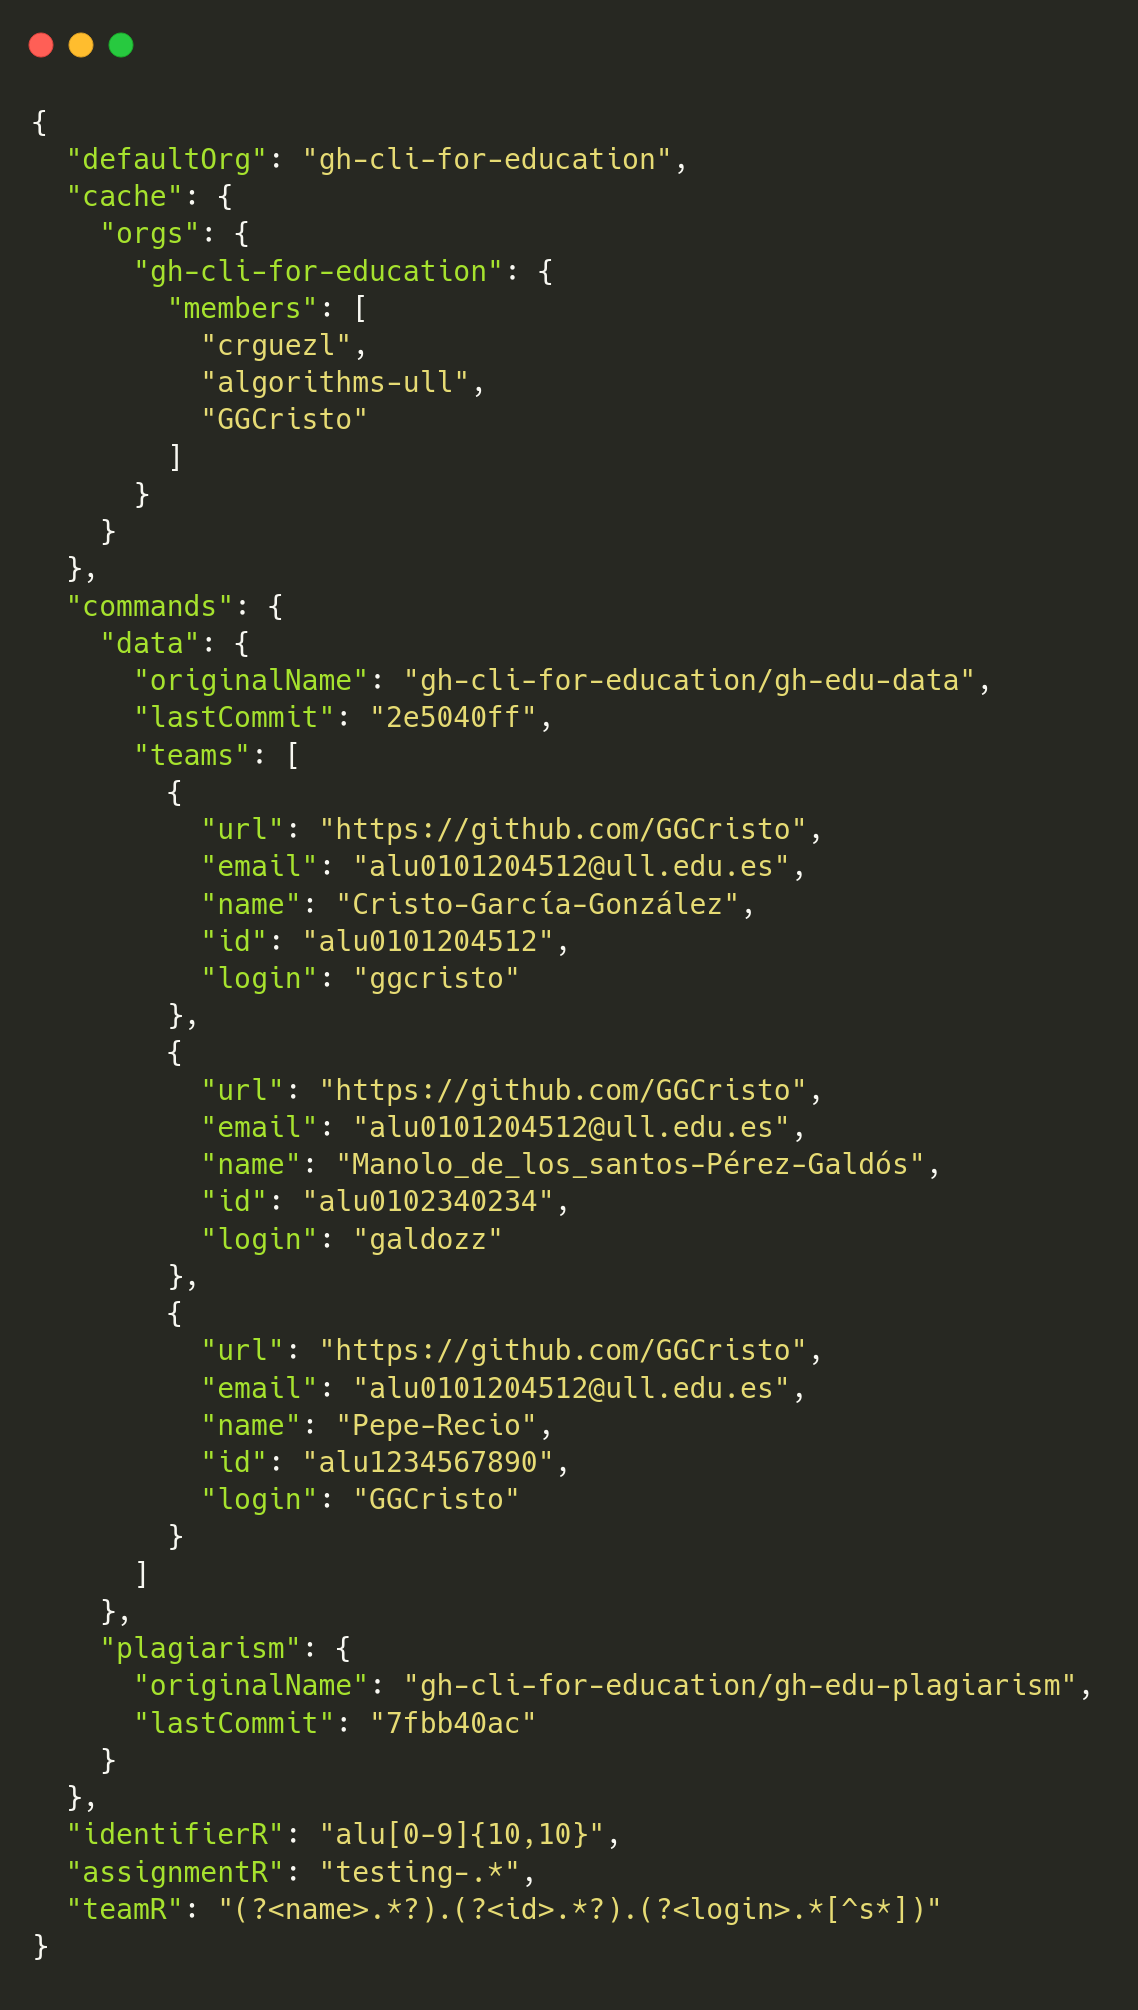
\includegraphics[height=0.5\paperheight]{images/data.png}}
    \caption{Ejemplo de data.json. El comando data tiene su propio campo: teams}
    \label{fig:data}
\end{figure}

El fichero \verb|data.json| es bastante importante. Se trata de un único fichero que actúa como memoria compartida para el intercambio de información entre el usuario, el core y las extensiones. Las extensiones no deben realizar operaciones de lectura, a excepción de una parte dedicada que tiene cada una para guardar sus propios datos (véase \ref{fig:data}). Cabe recordar que este fichero está ubicado en \verb|~/.config/gh-edu/data.json| en sistemas Unix y siempre está bajo gestión de versiones con \verb|Git|.

Tener todos los datos y configuraciones en un único fichero trae la ventaja de la portabilidad. Los usuarios pueden tener un repositorio privado con el nombre de \verb|gh-edu-profile| y así tener siempre una copia asegurada que puede utilizarse en diferentes máquinas.

El esquema mínimo necesario ya se pudo ver en la figura \ref{fig:configType}

\subsection{Integridad de los Datos}

Una extensión maliciosa o mal implementada podría corromper el fichero \verb|data.json|, afectando a otras extensiones. Al tratarse de un fichero, cualquier agente externo ya podía corromperlo, pero la probabilidad de que ocurra aumenta con el número y la calidad de las extensiones. Para intentar paliar esta posibilidad, siempre que se ejecute cualquier comando, el núcleo comprueba que \verb|data.json| es un fichero \verb|JSON| válido y la validez de sus campos (véase \ref{impl:gh-edu-data}). También en caso de error, si el error está relacionado por un campo incorrecto, como tener registrado una organización que no existe o a la cual no se pertenece, se muestra por pantalla el campo incorrecto que provocó el fallo. Junto al apoyo dado por el sistema de versiones, se espera que estas medidas sean suficientes para mejorar la robustez del sistema.


\subsection{Control del Versionado del Sistema}

Otra duda que surge de cara al futuro es como se va a controlar la evolución del controlador, de  \verb|data.json| y como las extensiones deberían reaccionar a dichos cambios. 
El problema surge cuando se introducen cambios en el controlador y el fichero \verb|data.json| que son incompatibles con el pasado. En tal caso el número de major de la versión  del controlador debería haberse incrementado.
Puede ocurrir entonces que una versión de una extensión/plugin de \verb|gh-edu| que funcionaba con una versión anterior del  controlador, deje de funcionar. 

El simple uso del \href{https://semver.org/lang/es/}{versionado semántico}, no resuelve el problema debido a la  posibilidad de un conflicto de dependencias en el que una extensión depende de una versión de \verb|data.json| en específico y otra extensión depende de una diferente. Normalmente con el versionado semántico se tienen las diferentes versiones necesarias de un mismo software, pero esa solución va en contra de la especificación de tener un único fichero. 


Obsérvese que el fichero \verb|data.json| contiene el número de versión semántica del controlador actual:

\begin{verbatim}
                    $ jq '.version' ~/.config/gh-edu/data.json 
                    "0.7.0"
\end{verbatim}

y que dicho número de versión puede ser consultado por cualesquiera extensiones para determinar su compatibilidad con el núcleo/{\emph core}.


En general se intentará mantener la retro-compatibilidad una vez el sistema alcance la estabilidad. Se romperá dicha compatibilidad únicamente en el caso de que sea estrictamente necesario para solucionar un error, notificando de esto a los desarrolladores de extensiones. El fichero \verb|data.json| se mantiene en un repositorio aparte bajo control de versiones. Esta característica debería facilitar la recuperación del sistema en caso de corrupción del fichero o error.


\subsection{El Manejo de la Localidad de los Datos: {\tt cache}}
Algunos comandos pueden llevar tiempo en ejecutarse, especialmente en organizaciones grandes. Es por eso que cierta información se guarda en la entrada \verb|cache| del fichero \verb|data.json| (véase  figura \ref{fig:configType}) y solo se busca y actualiza usando las \verb|API|s cuando la caché no tenga la información necesaria o el usuario desea actualizarla, lo que hará con el comando \verb|gh edu update -c|. 

La caché es un mecanismo de optimización algo peligroso si no se trata con cuidado, es por eso que las extensiones no deberían de escribir en ella. Las extensiones pueden implementar su propia caché en su propia zona asignada. Cabe mencionar que no todos los datos se almacenan en la caché, de momento solo los nombres de las organizaciones y los miembros pertenecientes a ellas son guardados. Se ha elegido estos datos y no otros porque muy rara vez una organización se elimina o renombra y lo mismo pasa con los alumnos o miembros de la organización.

\section{La Extensión gh-edu-plagiarism}
La extensión \verb|plagiarism| fue creada debido a que es uno de los tipos de extensión que más solicitan los profesores en el foro GitHub Classroom Community.

Se ha diseñado para que sea intuitivo y se puede usar tanto de forma interactiva como en un script, utilizando \verb|fzf| solo cuando los datos pasados por parámetros no son suficientes.

El servicio esencial de \verb|plagiarism| es \verb|MOSS|(Measure Of Software Similarity)\cite{MOSS} creado y ubicado en la universidad de Stanford. Se trata de un servicio que recibe código (en ficheros o directorios) y nos devuelve un enlace con un informe por cada combinación de pares posible. 
\begin{figure}
    \centering
    \makebox[\textwidth][c]{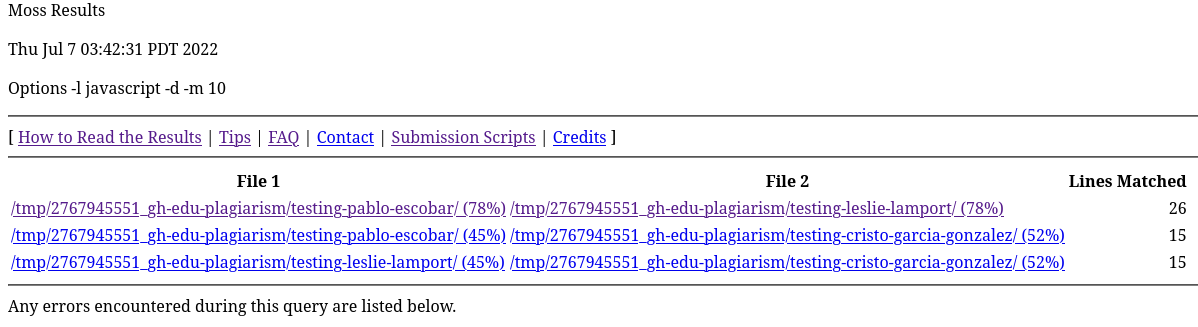
\includegraphics[width=\textwidth]{images/MOSS-raw.png}}
    \caption{Resultado de MOSS sin procesar}
    \label{fig:MOSSRaw}
\end{figure}

\verb|MOSS| es un servicio relativamente popular que lleva usándose desde 1994. Se eligió \verb|MOSS| por encima de otras tecnologías por varios motivos:
\begin{enumerate}
    \item \textbf{Compara cada tarea con el resto de tareas subidas.} Las alternativas comparan el código con código subido en internet. Algunos profesores no consideran plagio que ciertos fragmentos de código estén sacados de internet, incluso se llega a valorar positivamente.
    \item \textbf{Utiliza un algoritmo simple.} Que el algoritmo sea relativamente simple trae muchas ventajas. Por un lado, la ejecución es rápida, algo importante si tenemos en cuenta que se tiene que realizar \(\frac{n!}{(n-2)!2!}\) análisis. Por otro lado, los creadores afirman que después de años de servicio no se les ha informado de falsos positivos\cite{paper} (apartado 5.2 \verb|Plagiarism detection|).
    
    Un algoritmo simple también es suficiente para detectar técnicas comunes realizadas por los alumnos que se copian, como cambiar de nombre las variables, poner espacios en blanco o mover bloques de código de su posición original.
    Esta extensión fue creada para ayudar al profesor a concluir quien puede estar copiándose. No se debe confiar ciegamente en sus resultados.
\end{enumerate}

Otra dependencia menos importante es \verb|mossum|\cite{mossum}, un script hecho en \verb|python| que tiene como input \emph{n} links generados por \verb|MOSS| y que genera un grafo con los porcentajes de similitud entre las asignaciones.

La figura \ref{fig:plagiarism} muestra un diagrama de como funciona la extensión. Ha sido simplificado, ya que el código también se encarga de comprobar que se cumple con los requisitos, hace una configuración inicial y de forma paralela se comprueba en todo momento si ha ocurrido un error y se controla apropiadamente. Esto se conoce como \gls{graceful degradation} y específicamente intenta mostrar algún resultado, incluso si otro falla, en específico si no consigue devolver el informe ni el grafo, retornará un enlace, con una lista de reportes sin procesar, los mismos que devuelve el servidor de \verb|MOSS| (figura \ref{fig:MOSSRaw}).

\begin{figure}[H]
    \centering
    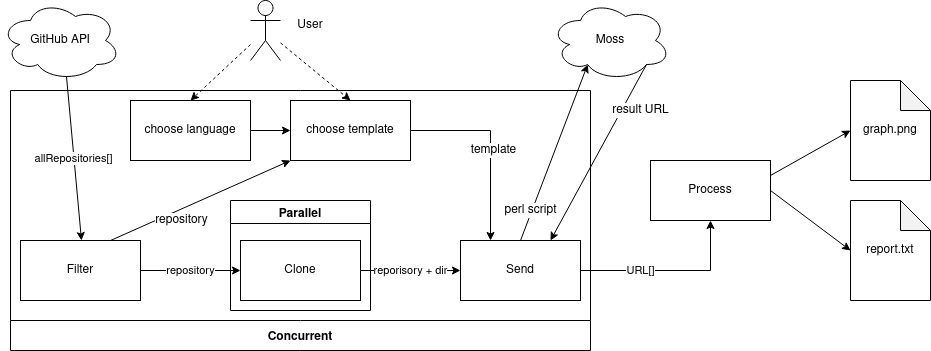
\includegraphics[width=\linewidth]{images/plagiarism.png}
    \caption{Diagrama de funcionamiento de plagiarism}
    \label{fig:plagiarism}
\end{figure}

Entrando en detalle, la aplicación 
\begin{enumerate}
    \item \textbf{GitHub API.} Empieza pidiendo todos los repositorios de la organización.
    \item \textbf{Filter.} Después pasa por un filtrado para quedarse con los repositorios que si interesan que sería aquellos relacionados con la tarea actual de la asignatura, utilizando expresiones regulares.
    \item \textbf{Clone.} Los repositorios se van clonando en paralelo en un directorio temporal del sistema.
    \item \textbf{Send.} A medida que se van clonando se les adjunta la dirección absoluta y se va preparando para ser enviados al servidor de \verb|MOSS| a través de su script.
    \item \textbf{Process.} Una vez \verb|MOSS| haya devuelto el enlace con los informes. ejecutamos el programa \verb|mossum| para la generación del grafo y la obtención del informe separado por pares de alumnos. Cuando el programa termina se muestra por pantalla un informe de todos los pares para que el profesor pueda ver las diferencias y determinar si de verdad hubo plagio (figura \ref{fig:reportPlagiarism}) y el susodicho grafo (figura \ref{fig:graphMossum}).
\end{enumerate}

Desde que el programa empieza se le pide al usuario información necesaria, en el caso de que no lo haya especificado por línea de comandos, como puede ser 
\begin{itemize}
    \item el lenguaje de programación utilizado en el código o
    \item una plantilla que el profesor haya proporcionado a los alumnos y sirva de base (en caso de haberla)
\end{itemize}

\begin{figure}[H]
    \centering
    \makebox[\textwidth][c]{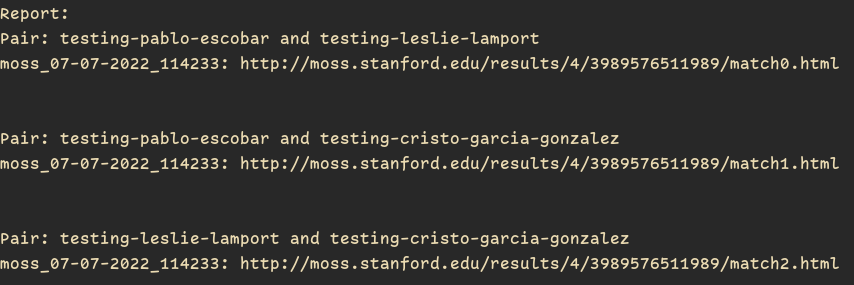
\includegraphics[width=\textwidth]{images/report-plagiarism.png}}
    \caption{Informe final dado por plagiarsim, con enlace para comprobar el código manualmente}
    \label{fig:reportPlagiarism}
\end{figure}

\begin{figure}[H]
    \centering
    \makebox[\textwidth][c]{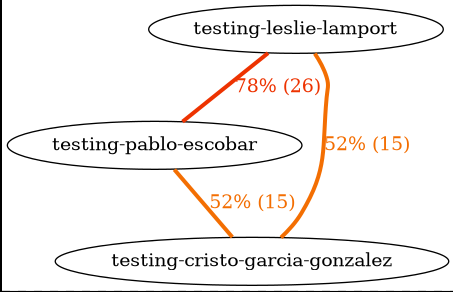
\includegraphics[width=0.5\textwidth]{images/grafo-moss.png}}
    \caption{Plagiarism. Grafo resultante mostrando los niveles de similitud}
    \label{fig:graphMossum}
\end{figure}

\emph{Nota: Debido a la política de privacidad de MOSS los informes pueden estar disponibles por 14 días, aunque también se avisa que existe la posibilidad de que se eliminen antes para poder liberar memoria de los servidores si se alcanza cierto límite no estipulado.}

La extensión \verb|plagiarism| funciona bastante bien con el sistema \verb|gh-edu|, pero también se ha diseñado para que sea posible su uso de forma independiente.


%%%%%%%%%%%%%%%%%%%%%%%%%%%%%%%%%%%%%%%%%%%%%%%%%%%%%%%%%
\newpage{\pagestyle{empty}}
\thispagestyle{empty}

\chapter{\LARGE Implementación}
\label{chapter:cuatro}

El objetivo de este capítulo es demostrar las partes importantes o de interés de la implementación y como se ha logrado la realización de lo estipulado en capítulos anteriores.

\section{El controlador}
Como se ha comentado en capítulos anteriores, la mayoría de comandos se aprovecha de los comandos ya proporcionados por \verb|gh|. Como es el caso de \verb|gh edu install|. Después de determinar si la extensión es \emph{first-party} o \emph{third-party} (extensión independiente de la organización \verb|gh-cli-for-education|), se obtiene la dirección del repositorio de la extensión, se invoca \verb|gh extension install| y se añade a \verb|data.json|.

\begin{figure}[H]
    \centering
    \makebox[\textwidth][c]{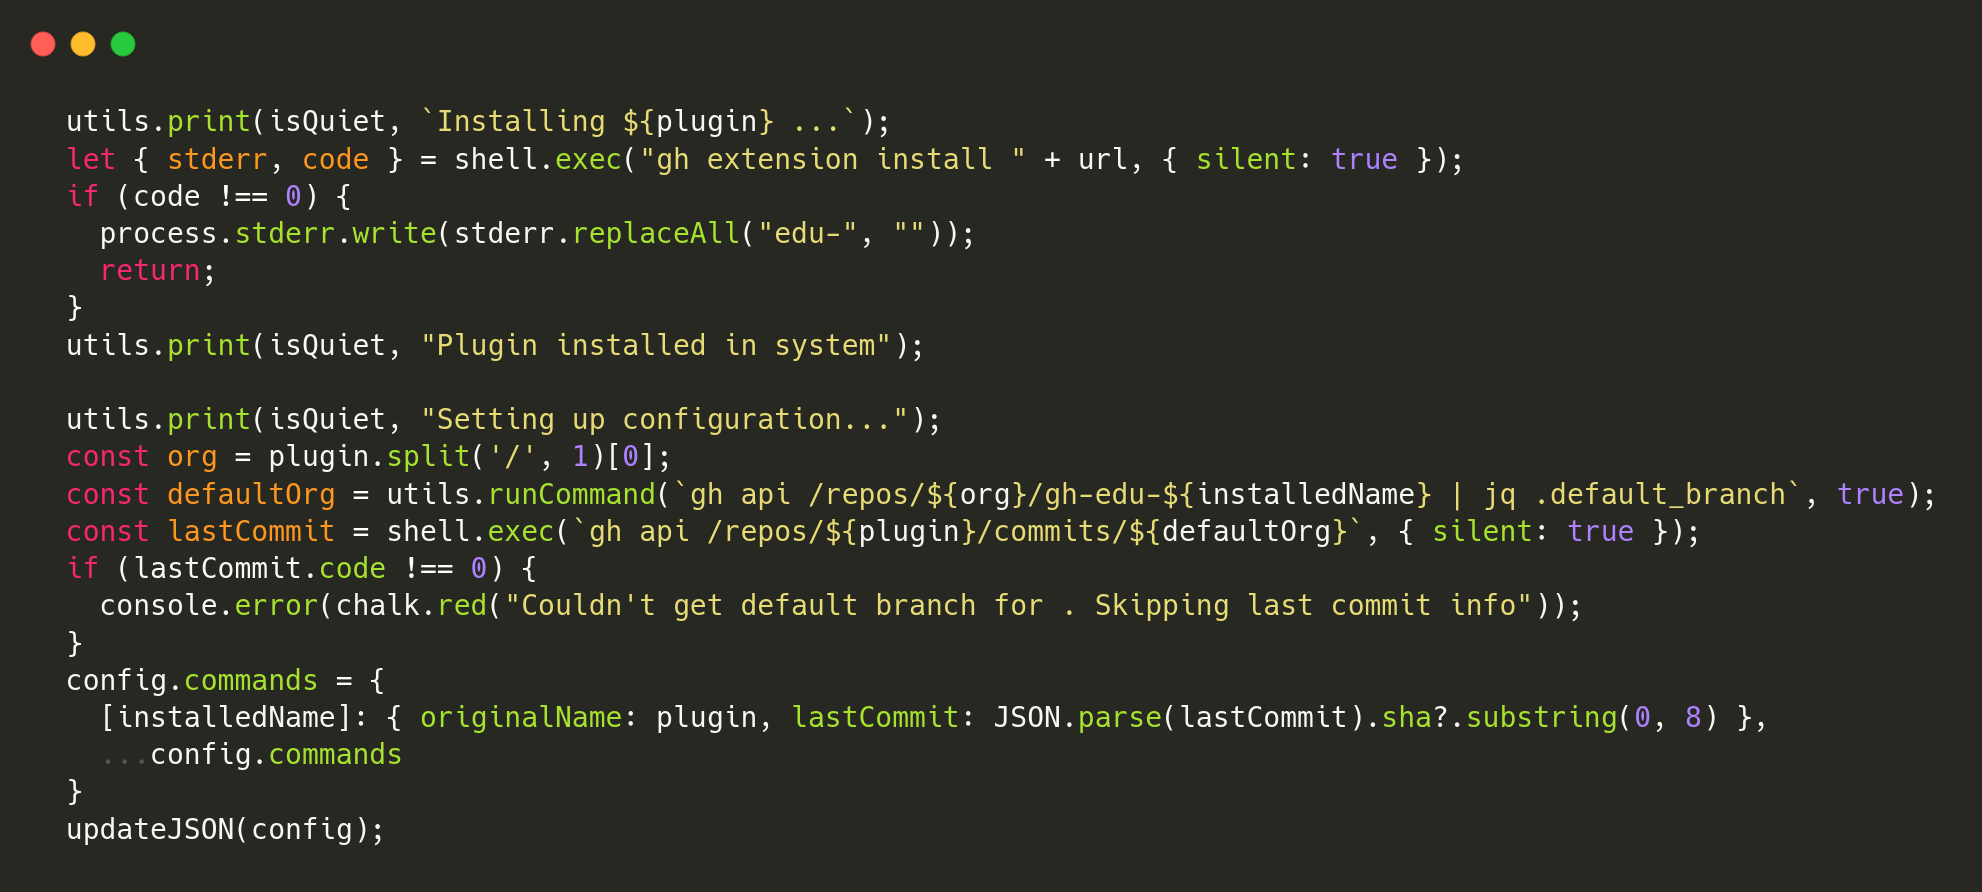
\includegraphics[width=\textwidth]{images/installCode.png}}
    \caption{Implementación. Código para instalar extensiones}
    \label{fig:installCode}
\end{figure}

En la figura \ref{fig:installCode} vemos que después de instalar la extensión, hacemos una llamada \emph{API REST} para saber cuál es la rama por defecto. Al tener esta información, podemos buscar cuál es el \gls{hash} del último \emph{commit}, para actualizar el campo \verb|lastCommit|.

\emph{Nota: utils.print() es una función muy simple para determinar si el mensaje debería imprimirse o no, dependiendo del valor del flag --quiet}.

Para que \verb|commander| acepte únicamente las extensiones instaladas, se ha escrito el siguiente código (figura \ref{fig:addThirdParty}):

\begin{figure}[H]
    \centering
    \makebox[\textwidth][c]{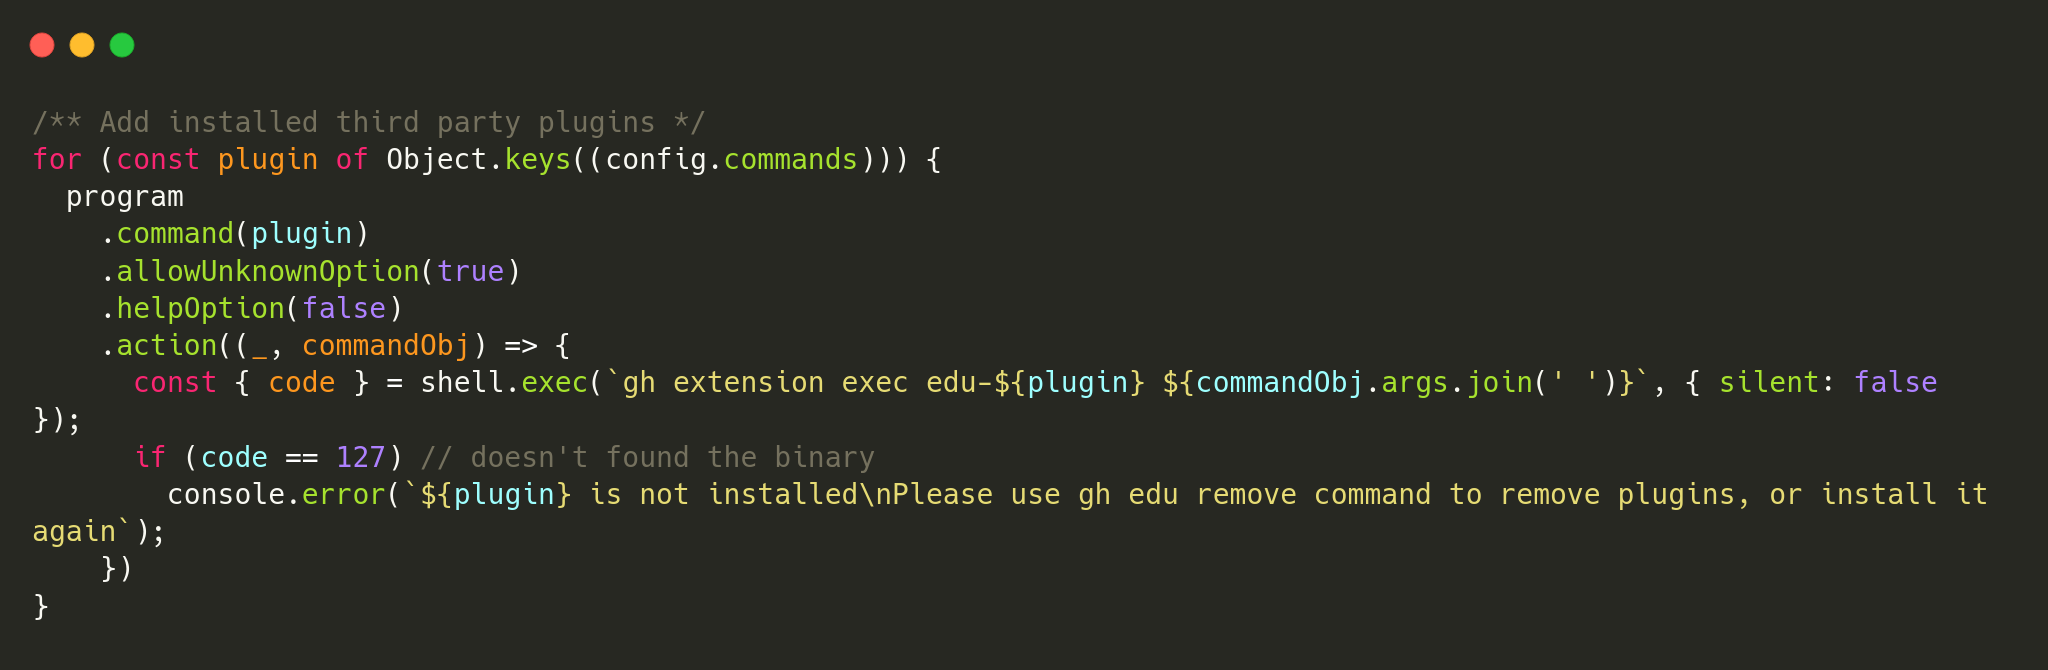
\includegraphics[width=\textwidth]{images/addThirdParty.png}}
    \caption{Implementación. Controlador. Añadir extensiones third-party}
    \label{fig:addThirdParty}
\end{figure}

Todas las extensiones, que se hayan instalado en el sistema a través de \verb|gh-edu|, se añadirán como comandos disponibles. También se activa la posibilidad de usar opciones desconocidas y se delega su gestión al subcomando en cuestión. Así mismo se desactiva la ayuda y en el manejo de errores solo se comprueba que el comando haya sido ejecutado, pues naturalmente de estas tareas se tiene que ocupar cada extensión.

Aquí se deja ver la madurez del programa al permitirnos utilizar comandos desconocidos, función que, al momento de escribir estas líneas, todavía no es posible con \href{https://github.com/spf13/cobra/issues/739}{cobra}.

\subsection{Manejo del único punto de información: data.json} \label{impl:data.json}
Lo primero que el programa hace al ser ejecutado, es comprobar la validez del fichero. La siguiente figura (\ref{fig:dataGraph}) muestra los estados por los que se pasa para lograrlo.

\begin{figure}[H]
    \centering
    \makebox[\textwidth][c]{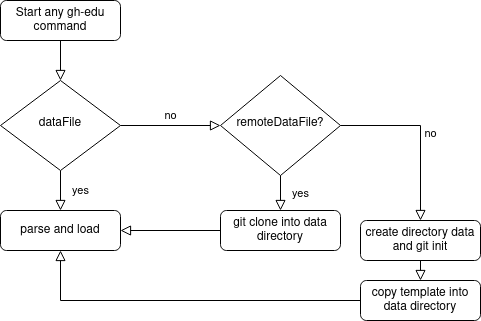
\includegraphics[width=0.5\textwidth]{images/createConfig.png}}
    \caption{Obtención del archivo data.json}
    \label{fig:dataGraph}
\end{figure}

Es primer paso es comprobar si se encuentra en la localización correspondiente (\verb|~/.config/gh-edu/data.json|). De no ser así, se intenta conseguirlo desde el repositorio \verb|gh-edu-profile|. Como última instancia se crea un fichero nuevo, partiendo de una plantilla que contiene todos los campos necesarios.

Sabiendo que el fichero está disponible, pasamos a validar su contenido. Primero se \glspl{deserialization} para comprobar que es un fichero JSON válido. Acto seguido pasamos a realizar una comprobación simple de los campos, comprobando que estén en el fichero y que las \glspl{regex} sean válidas.

\begin{figure}[H]
    \centering
    \makebox[\textwidth][c]{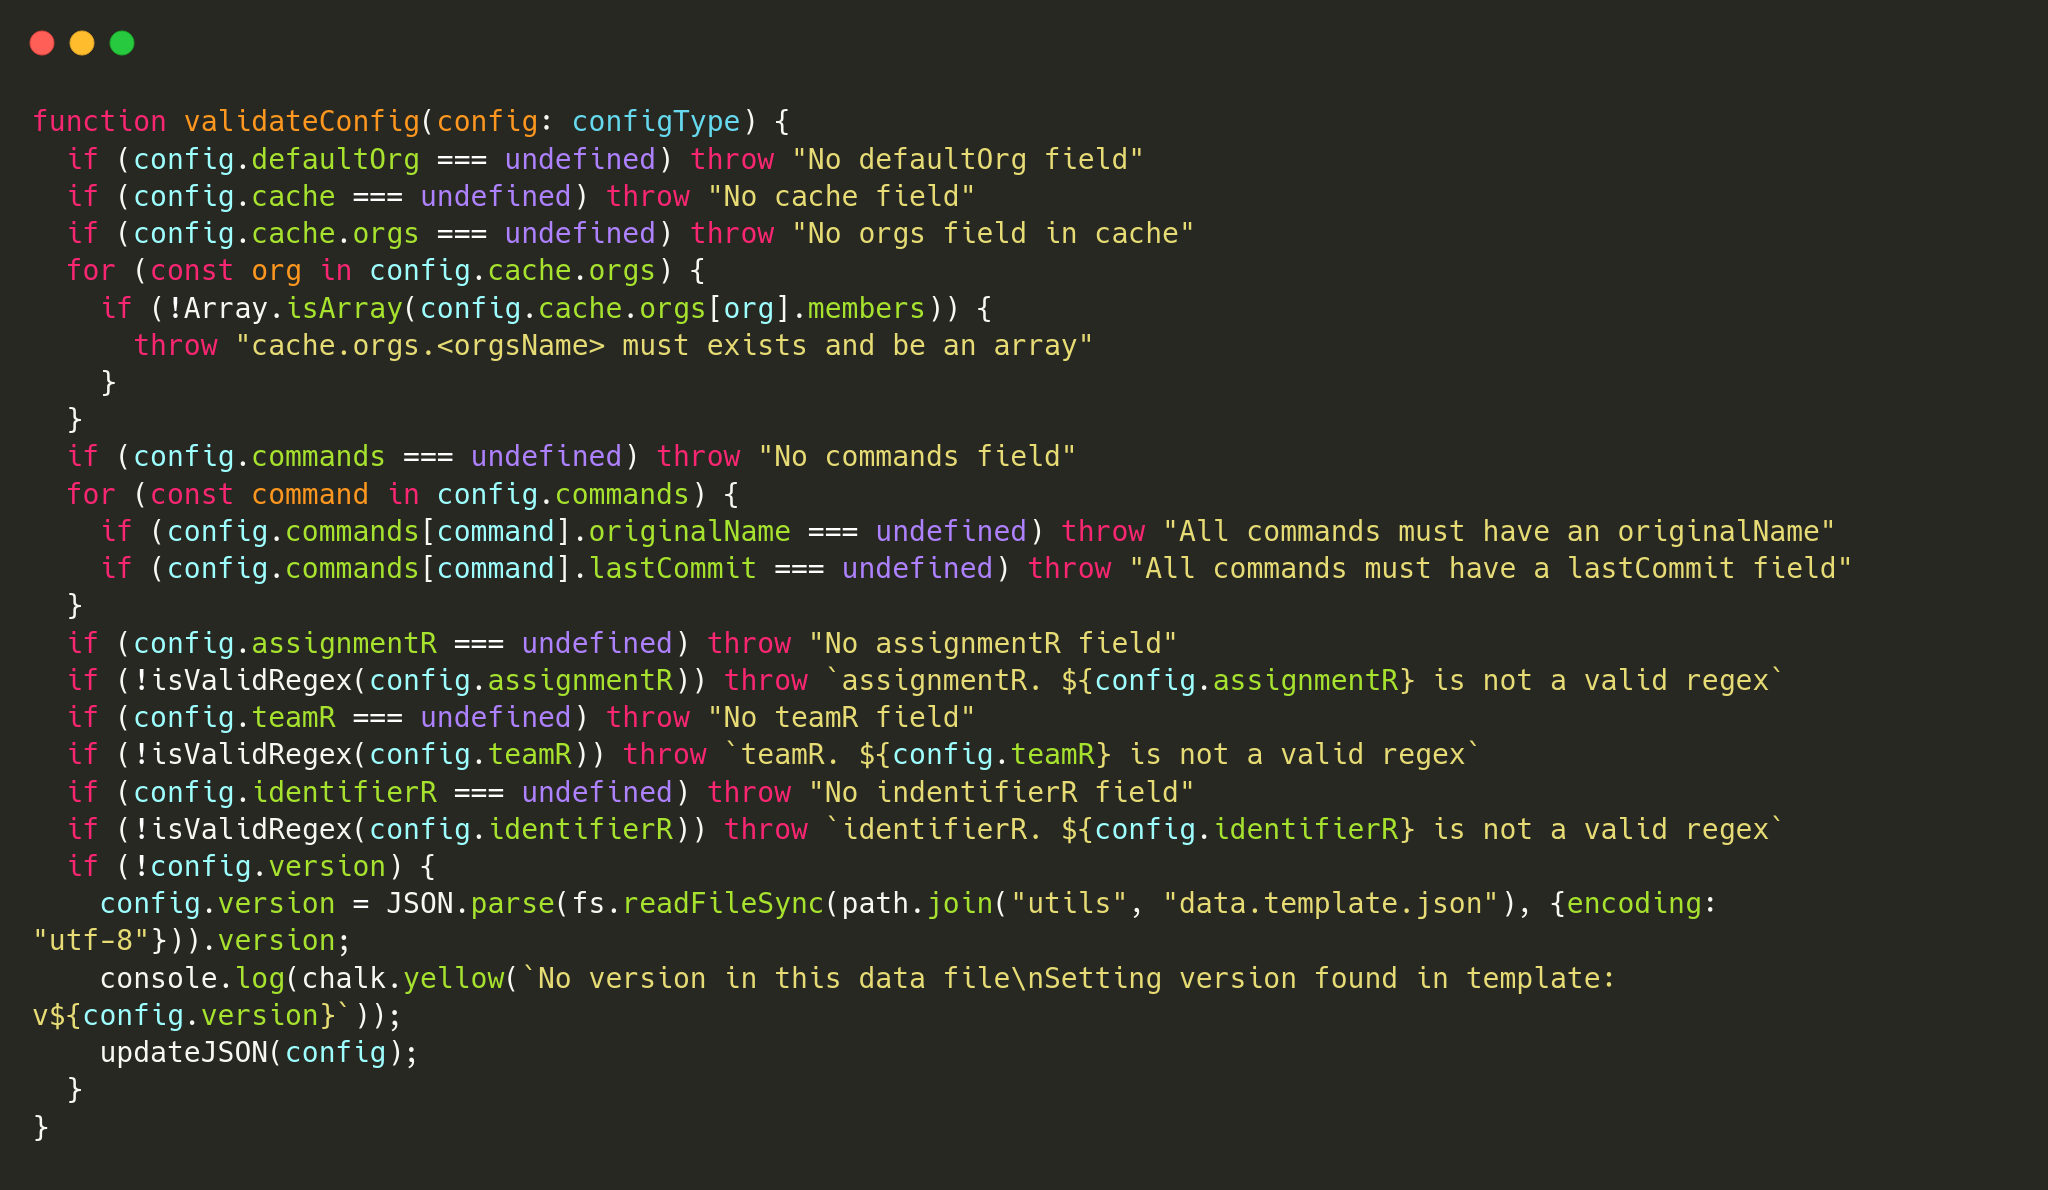
\includegraphics[width=\textwidth]{images/comprobacion.png}}
    \caption{Implementación. data.json. Comprobamos que los campos son válidos}
    \label{fig:comprobar}
\end{figure}

Cada vez que se quiera actualizar la información, se actualiza la variable donde se cargó el fichero, se \glspl{serialization} y se escribe de vuelta al fichero.

\section{Extensión minimalista: {\tt gh-edu-view}}\label{sec:gh-edu-view-implementation}

A la hora de escribir una extensión para \verb|gh-edu| en \verb|JS|, se procede de la misma forma que con una extensión \verb|gh|.
Deben crearse los ficheros \verb|gh-edu-view/gh-edu-view| (script bash) y \verb|gh-edu-view/gh-edu-view.js| (programa \verb|JS|).

Para intentar conseguir los identificadores relacionados a los alumnos, con nada más que la información proporcionada con GitHub, no nos queda otra opción que buscar en todos los campos, donde dicha información podría estar disponible, y devolver un \emph{array} con todos los posibles resultados.

\begin{figure}[H]
    \centering
    \makebox[\textwidth][c]{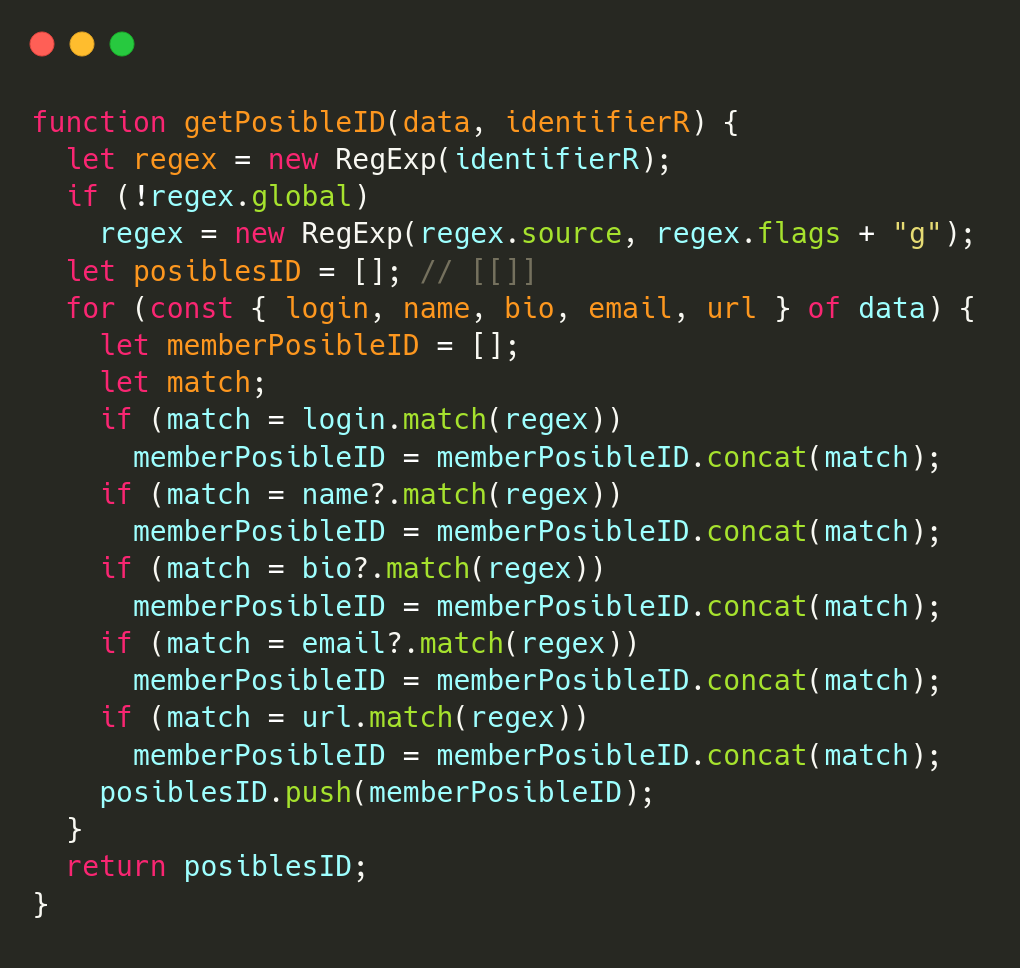
\includegraphics[width=0.5\textwidth]{images/posibleID.png}}
    \caption{Implementación. gh-edu-view. Obtención de posibles identificadores}
    \label{fig:viewId}
\end{figure}

Toda la información proporcionada por el comando \verb|members| se puede conseguir con una simple petición en GraphQL (figura \ref{fig:viewQuery}).

\begin{figure}[H]
    \centering
    \makebox[\textwidth][c]{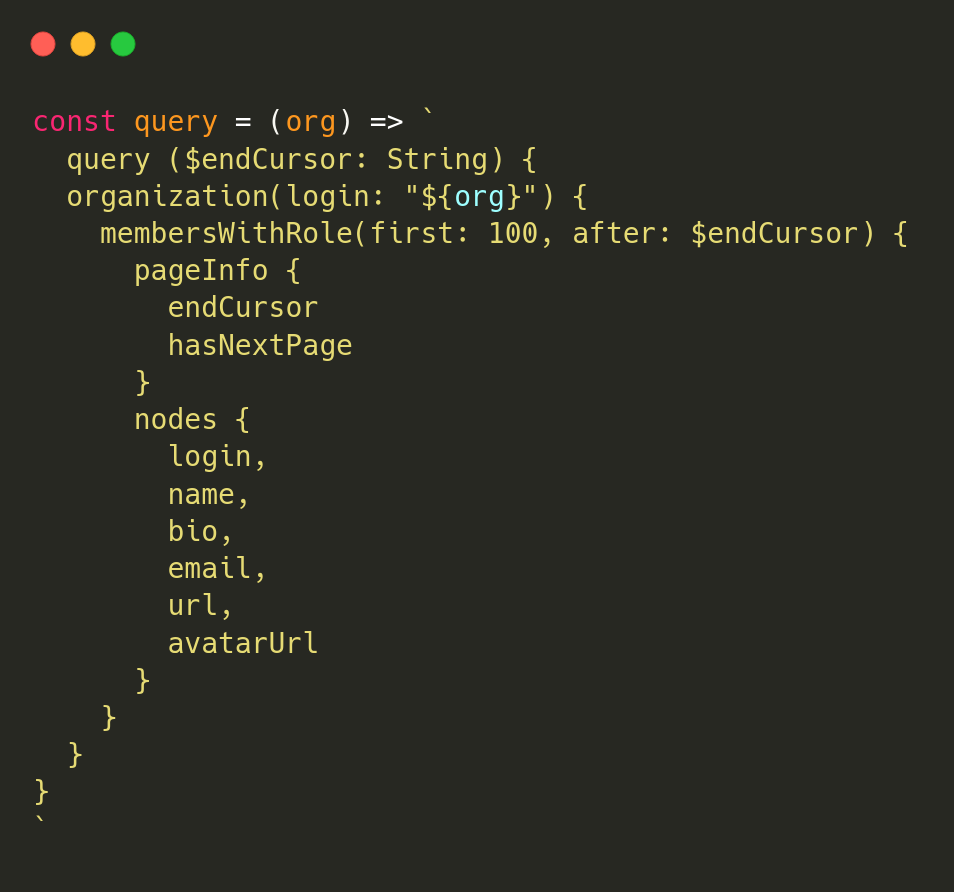
\includegraphics[width=0.5\textwidth]{images/view-query.png}}
    \caption{Implementación. gh-edu-view. Petición para conseguir diversos campos de cada alumno}
    \label{fig:viewQuery}
\end{figure}

\section{{La librería \tt shelljs} y el manejo de E/S: {\tt gh-edu-data}} \label{impl:gh-edu-data}
Uno de los defectos de \verb|shelljs| que ya se ha comentado en el apartado de \textbf{Tecnologías} (\ref{shelljs}) es como no permite el uso de \verb|STDIN| o tuberías. Algo importante en este proyecto, pero especialmente en esta extensión por el uso avanzado de \verb|fzf| y \verb|jq|. Estas dos tecnologías, a pesar de ser completamente independientes la una a la otra, pueden trabajar conjuntamente gracias a su diseño flexible y minimalista a través de tuberías, haciendo posible la previsualización dinámica de los elementos en el comando \verb|log| (figura \ref{fig:interface-log})

Este comportamiento es requerido, ya que no es posible pasar un objeto \verb|JS| o un \emph{array} al input de un programa que todavía no ha sido ejecutado. Solo se puede usar cadenas de texto. Lo ideal es ejecutar el comando, y de forma asíncrona ir procesando la estructura de datos, enviando cadenas de texto, como se hace en \verb|gh-edu-plagiarism| (gracias a \href{https://pkg.go.dev/os/exec@go1.18.3#Cmd.StdinPipe}{cmd.StdInPipe}).

Hasta que la \href{https://github.com/shelljs/shelljs/issues/424}{incidencia 424} no sea resuelta, se ha tenido que realizar una solución alternativa utilizando ficheros temporales. La idea consiste en formatear el objeto o \verb|array| y escribir el resultado en un fichero, de esta forma podemos leer el fichero y transmitir esa información por medio de una tubería a otro comando en el mismo momento en el que se ejecuta el comando.

\section{Concurrencia con Go y CSP: {\tt gh-edu-plagiarism}} \label{diseño:gh-edu-plagiarism}
A diferencia del resto de extensiones \verb|plagiarism| está implementado en Go. Uno de los motivos del cambio de lenguaje es demostrar como se puede desarrollar extensiones en cualquier lenguaje sin muchas dificultades.

También, como se comentó en \textbf{Tecnologías} (\ref{go}) este programa es altamente concurrente y paralelo. Go cuenta con un modelo de concurrencia bastante particular basado en el trabajo teórico de Tony Hoare \emph{Communicating Sequential processes} (CSP) \cite{hoare1985communicating}.

Para entender las explicaciones de esta sección es necesario conocer dos conceptos: las gorutinas y los canales. Las gorutinas son \glspl{corrutine} independientes que se ejecutan en hilos verdes (\emph{green threads}), los cuales son hilos emulados generados en tiempo de ejecución, estos hilos se multiplexan a hilos reales del procesador a través del \verb|Go scheduler|, que determina cuanto tiempo debe estar cada hilo verde consumiendo CPU.

Los canales son la estructura de datos que nos permite enviar información de una gorutina a otra y también sirven de elemento sincronizador, cuando se envía un elemento, la gorutina no continua hasta que el otro lado (el emisor) haya recibido la información y viceversa.

La explicación de la figura \ref{fig:plagiarism} en términos de código sería la siguiente:\\
Cada bloque dentro del módulo \verb|Concurrent| es una gorutina que se ejecuta de forma independiente y cada flecha pertenece a un canal, que sincroniza y a su vez transmite información de una gorutina a otra.

La gorutina \verb|clone| va creando a su vez gorutinas a medida que más repositorios se vayan filtrando. Debido a que las gorutinas apenas consumen recursos, está bien eliminar y crear tantas como queramos. No obstante, como estamos realizando programación paralela, tenemos que tener cuidado de que no haya muchas más gorutinas corriendo que núcleos disponibles en el procesador, pues entonces conseguiríamos el efecto contrario al deseado, ralentizando toda la aplicación debido al constante cambio de contexto entre hilos. Para limitar la creación de gorutinas al número de núcleos disponibles se ha utilizado un semáforo. Un semáforo es una variable o estructura de datos que permite una cantidad arbitraria de procesos. Un semáforo binario es a efectos prácticos un \verb|lock| o \verb|mutex|.

\begin{figure}[H]
    \centering
    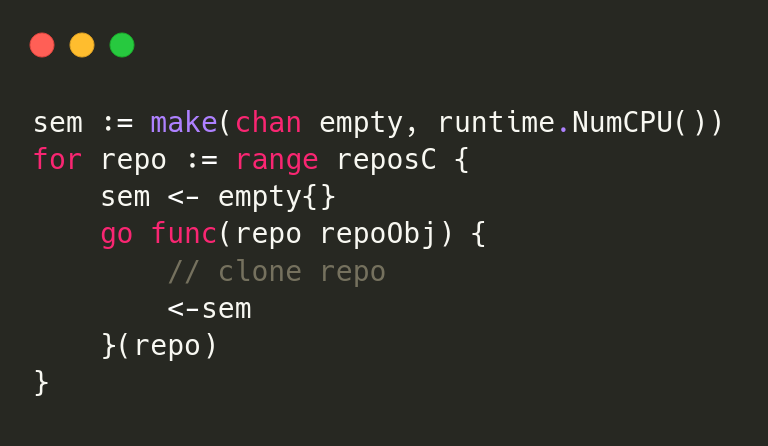
\includegraphics[width=0.5\linewidth]{images/concurrency-go.png}
    \caption{Paralelismo limitado con un sémaforo}
    \label{fig:concurrencyGo}
\end{figure}
El código que lo implementa (figura \ref{fig:concurrencyGo}) ha sido simplificado para explicar el funcionamiento del paralelismo y el semáforo.

El canal \verb|sem| es un canal con buffer, esto quiere decir que no para el flujo (no sincroniza) hasta que el buffer se llene. El tamaño de dicho buffer es \verb|runtime.NumCPU()| que retorna el número de núcleos disponibles al ejecutar el programa. En cada iteración del bucle \verb|repo| contiene un nuevo repositorio proveniente del módulo \verb|Filter| y enviamos un elemento al canal \verb|sem|, el elemento en cuestión es irrelevante, estamos usando el canal por sus propiedades de sincronización, no para la transferencia de datos. Después ejecutamos una gorutina anónima que se encarga de clonar el repositorio, cuando termine escucha y descarta del canal \verb|sem|.

De esta forma, si \verb|sem| está lleno significa que ya hay tantos procesos ejecutándose como núcleos hay disponibles, por lo que el programa queda en espera hasta que quede un hueco en el semáforo.

% Esto va en diseño. Otro de los motivos por los cuales se eligió Go es que a la hora de diseñar la extensión me percate de que el programa sería altamente concurrente y paralelo. Uno de los motivos por los cuales se creó Go fue para poder aprovechar al máximo los varios núcleos que suele tener cualquier dispositivo moderno. Así, las instituciones educativas que reutilizan la misma organización para una misma asignatura a lo largo de varios años, y por ende tienen muchos repositorios y miembros, no verán su experiencia lastrada. También se tuvo en cuenta que Go tiene soporte de primera clase con \verb|gh| y uno de los casos de uso más comunes del lenguaje son aplicaciones CLI.

\begin{figure}[H]
    \centering
    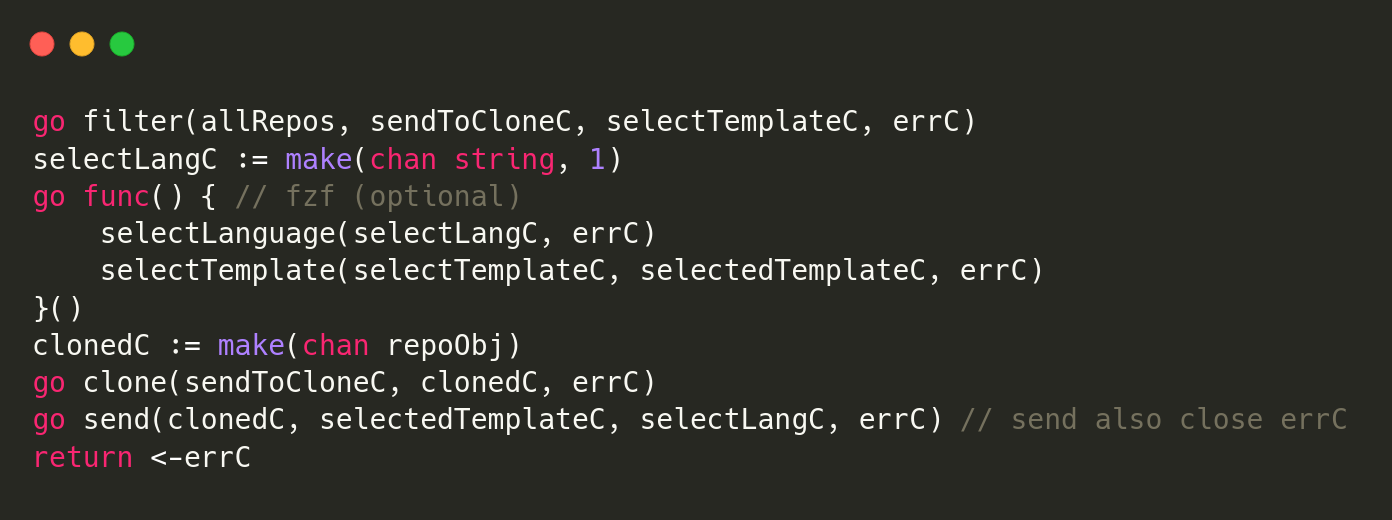
\includegraphics[width=\linewidth]{images/go-code.png}
    \caption{Código general de plagiarism}
    \label{fig:goCode}
\end{figure}

 

%%%%%%%%%%%%%%%%%%%%%%%%%%%%%%%%%%%%%%%%%%%%%%%%%%%%%%%%%
\newpage{\pagestyle{empty}}
\thispagestyle{empty}

\chapter{\LARGE Conclusiones y líneas futuras}
\label{chapter:Resultados}

``Software Engineering Is Programming Integrated Over Time'' \label{conclusion}

\bigskip
Lo que más resalto en este trabajo de fin de grado ha sido la tarea de diseñar un ecosistema modulable desde cero con unas metas marcadas y con el ideal de crear un software que no necesite de cambios en su estructura para crecer, que sea simple e intuitivo, pero útil y que permita la colaboración. Conseguir todas estas características ha requerido una amplia etapa de diseño y prototipado donde las ideas se implementaban y descartaban por igual.\\
También otro apartado que consumió bastante tiempo fue el manejo de errores. Al ser una aplicación que realiza muchas llamadas, lee y escribe de ficheros y le pide \emph{input} al usuario, hay muchos puntos donde la aplicación puede fallar. Manejar estos errores y pulir la aplicación en general es trabajo que no genera un resultado inmediato, pero hace que la aplicación sea más mantenible y estable.\\
Por otro lado, me siento muy afortunado de haber podido trabajar con tecnologías con las que me siento cómodo como JavaScript, Go y \verb|fzf|, pero han sido más las que he aprendido y dada la buena experiencia que he tenido con: \verb|jq|, \verb|gh cli| y \verb|GraphQL| comentar que seguramente las utilice en futuros proyectos.\\
No obstante, me apena no haber podido cumplir con el objetivo de interoperabilidad entre comandos. El comando \verb|view| se podría beneficiar enormemente si pudiese leer de la \emph{standard input} para recibir información de un comando como \verb|data|, pero preferí enfocar el tiempo en mejorar la calidad y usabilidad de todo el ecosistema.\\
El trabajo de fin de grado está terminado, pero el proyecto puede crecer tanto como desee. Este tipo de proyecto requiere de trabajo constante y prolongado para que tenga acogida en la comunidad. Mis intenciones son seguir contribuyendo a este proyecto y tomarlo como mi proyecto personal y mi vía de contribución al open source.

%%%%%%%%%%%%%%%%%%%%%%%%%%%%%%%%%%%%%%%%%%%%%%%%%%%%%%%%%
\newpage{\pagestyle{empty}}
\thispagestyle{empty}

\chapter{\LARGE Summary and Conclusions}
\label{chapter:Conclusiones}

``Software Engineering Is Programming Integrated Over Time''

\bigskip


%%%%%%%%%%%%%%%%%%%%%%%%%%%%%%%%%%%%%%%%%%%%%%%%%%%%%%%%%
\newpage{\pagestyle{empty}}
\thispagestyle{empty}

\chapter{\LARGE Presupuesto}
\label{chapter:presupuesto}

Todas las tecnologías usadas son \emph{open source} y gratuitas y se presupone que el ordenador usado es personal, por lo que no se incluye en el presupuesto\\
El hipotético saldo son 15 euros la hora

\begin{comment}
\begin{center}
\begin{tabu} to 0.8\textwidth {| X[l] | X[l] | X[l] |}
 \hline
 \multicolumn{1}{|c|}{\bf Coste} & \multicolumn{1}{|c|}{\bf Tipos} & \multicolumn{1}{|c|}{\bf Descripción} \\
 \hline 4500 & Formación y Diseño & La formación en nuevas tecnologías y el diseño de la aplicación han consumido un tiempo sustancial de 300 horas\\
 \hline
 3000  & Desarrollo de los prototipos y aplicación final & Aproximadamente se ha dedicado unas 200 horas\\
 \hline
 120 & Elaboración del informe y conclusiones  & Al tratarse de un ecosistema \emph{open source} lanzado a un público general, la documentación es importante, por lo que se ha desarrollado no solo este informe. si no documentación para usuario y desarrolladores en los respectivos repositorios. \\
 \hline
\end{tabu}
\end{center}
\end{comment}
\begin{table}[H]
    \centering
    \begin{tabular}{|m{1cm}|m{4cm}|m{10cm}|}
    \hline
    \textbf{Coste} & \textbf{Tipos} & \textbf{Descripción}\\
    \hline
    4500 & Diseño y planificación & Incluyendo el tiempo invertido en investigación de las nuevas tecnologías necesarias y el diseño y planificación de la aplicación se ha consumido un tiempo sustancial de 300 horas\\
    \hline
    3000  & Desarrollo de los prototipos y aplicación final & Aproximadamente se ha dedicado unas 200 horas\\
    \hline
    495 & Elaboración del informe y conclusiones  & Al tratarse de un ecosistema \emph{open source} lanzado a un público general, la documentación es importante, por lo que se ha desarrollado no solo este informe. si no documentación para usuario y desarrolladores en los respectivos repositorios. Necesitando un total de 33 horas\\
    \hline
    \end{tabular}
    \caption{Tabla del presupuesto}
    \label{tab:budget}
\end{table}

\begin{comment}
   \begin{table}[htb]
   \centering
   \caption{Presupuesto}
   \label{table:presupuesto}
\end{table} 
\end{comment}

Esto supone un presupuesto total de, 7995 euros en un periodo de 3 meses

%%%%%%%%%%%%%%%%%%%%%%%%%%%%%%%%%%%%%%%%%%%%%%%%%%%%%%%%%
\newpage{\pagestyle{empty}\cleardoublepage}
\thispagestyle{empty}

\begin{appendix}

\chapter{\LARGE Repositorios del ecosistema}
\label{appendix:1}
Se adjuntan los enlaces a los repositorios de GitHub de los diferentes códigos en los que se ha trabajado.

\begin{itemize}
  \item XXXX
  El código de \verb|gh-edu| se encuentra en

  \href{https://github.com/gh-cli-for-education/gh-edu}{{\tt https://github.com/gh-cli-for-education/gh-edu}}

  
\end{itemize}

\end{appendix}
%\printnoidxglossaries
\printglossary[title=Glosario, toctitle=Glosario]

%%%%%%%%%%%%%%%%%%%%%%%%%%%%%%%%%%%%%%%%%%%%%%%%%%%%%%%%%%
%\begin{thebibliography}{X}
% Aquí figurará la bibliografía
%\end{thebibliography}
%\bibliographystyle{plain}
\bibliographystyle{unsrt}

\bibliography{memtfg} 
%\bibliography{bib.tex}
%%%%%%%%%%%%%%%%%%%%%%%%%%%%%%%%%%%%%%%%%%%%%%%%%%%%%%%%%%

\end{document}

